% **************************************************
% Document Class Definition
% **************************************************
\documentclass[%
    paper=A4,               % paper size --> A4 is default in Germany
    twoside=false,          % onesite or twoside printing
    openright,              % doublepage cleaning ends up right side
    parskip=half*,          % spacing value / method for paragraphs
    chapterprefix=true,     % prefix for chapter marks
    11pt,                   % font size
    headings=normal,        % size of headings
    bibliography=totoc,     % include bib in toc
    listof=totoc,           % include listof entries in toc
    titlepage=on,           % own page for each title page
    captions=tableabove,    % display table captions above the float env
    chapterprefix=false,    % do not display a prefix for chapters
    appendixprefix=false,   % but display a prefix for appendix chapter
    draft=false,            % value for draft version
]{scrreprt}%


% **************************************************
% Setup YOUR thesis document in this file !
% **************************************************
% !TEX root = main.tex


% **************************************************
% Files' Character Encoding
% **************************************************
\PassOptionsToPackage{utf8}{inputenc}
\usepackage{inputenc}


% **************************************************
% Information and Commands for Reuse
% **************************************************
\newcommand{\thesisTitle}{Simplifying NeRF: Creating an Intuitive Web-Based 3D Scene Interface}
\newcommand{\thesisName}{Eduard Aurelius von Briesen Brandenburg Neumark}
\newcommand{\thesisSubject}{Master`s Thesis}
\newcommand{\thesisDate}{\today}
\newcommand{\thesisVersion}{0.1}

% \newcommand{\thesisFirstReviewer}{Eyke H{\"u}llermeier}
% \newcommand{\thesisFirstReviewerUniversity}{\protect{LMU Munich}}
% \newcommand{\thesisFirstReviewerDepartment}{Institute of Informatics}

\newcommand{\thesisFirstSupervisor}{Prof. Dr. Sylvia Rothe}
\newcommand{\thesisSecondSupervisor}{Christoph Johannes Weber}

\newcommand{\thesisUniversity}{LMU Munich}
\newcommand{\thesisUniversityDepartment}{Department of Mathematics, Informatics and Statistics}
\newcommand{\thesisUniversityInstitute}{Institute of Informatics}
\newcommand{\thesisUniversityGroup}{}
\newcommand{\thesisUniversityCity}{Munich}
\newcommand{\thesisUniversityStreetAddress}{Akademiestra\ss e 7}
\newcommand{\thesisUniversityPostalCode}{80799 Munich}


% **************************************************
% Debug LaTeX Information
% **************************************************
%\listfiles

% **************************************************
% Load and Configure Packages
% **************************************************
\usepackage[english]{babel} % babel system, adjust the language of the content
\PassOptionsToPackage{% setup clean thesis style
    figuresep=colon,%
    hangfigurecaption=false,%
    hangsection=true,%
    hangsubsection=true,%
    sansserif=false,%
    configurelistings=true,%
    colorize=full,%
    colortheme=lmuaiml,%
    configurebiblatex=true,%
    bibsys=bibtex,%
    bibfile=bib-refs,%
    bibstyle=numeric,%
    bibsorting=nty,%
}{cleanthesis}
\usepackage{cleanthesis}

\usepackage{mathtools}

\hypersetup{% setup the hyperref-package options
    pdftitle={\thesisTitle},    %   - title (PDF meta)
    pdfsubject={\thesisSubject},%   - subject (PDF meta)
    pdfauthor={\thesisName},    %   - author (PDF meta)
    plainpages=false,           %   -
    colorlinks=false,           %   - colorize links?
    pdfborder={0 0 0},          %   -
    breaklinks=true,            %   - allow line break inside links
    bookmarksnumbered=true,     %
    bookmarksopen=true          %
}

% **************************************************
% Other Packages
% **************************************************
\usepackage{scrhack}
\usepackage{lipsum}
\usepackage{tikz}% do not disable this package

\usetikzlibrary{backgrounds,calc}

\usepackage{pgf-pie}
\usepackage{tabularx}
\usepackage{listings}
\usepackage{subcaption}
\usepackage{todonotes}
\usepackage{wrapfig}
\usepackage{pgfplots}
\pgfplotsset{compat=1.17}


\usepackage[top=3cm,left=3cm,right=3cm,bottom=4cm]{geometry}

\lstdefinelanguage{JavaScript}{
  morekeywords=[1]{break, continue, delete, else, for, function, if, in,
    new, return, this, typeof, var, void, while, with},
  % Literals, primitive types, and reference types.
  morekeywords=[2]{false, null, true, boolean, number, undefined, string,
    Array, Boolean, Date, Math, Number, String, Object},
  % Built-ins.
  morekeywords=[3]{eval, parseInt, parseFloat, escape, unescape},
  sensitive,
  morecomment=[s]{/*}{*/},
  morecomment=[l]//,
  morecomment=[s]{/**}{*/}, % JavaDoc style comments
  morestring=[b]',
  morestring=[b]"
}[keywords, comments, strings]

\lstalias[]{ES6}[ECMAScript2015]{JavaScript}

\lstdefinelanguage[ECMAScript2015]{JavaScript}[]{JavaScript}{
  morekeywords=[1]{await, async, case, catch, class, const, default, do,
    enum, export, extends, finally, from, implements, import, instanceof,
    let, static, super, switch, throw, try},
  morestring=[b]` % Interpolation strings.
}

% Requires package: color.
\definecolor{mediumgray}{rgb}{0.3, 0.4, 0.4}
\definecolor{mediumblue}{rgb}{0.0, 0.0, 0.8}
\definecolor{forestgreen}{rgb}{0.13, 0.55, 0.13}
\definecolor{darkviolet}{rgb}{0.58, 0.0, 0.83}
\definecolor{royalblue}{rgb}{0.25, 0.41, 0.88}
\definecolor{crimson}{rgb}{0.86, 0.8, 0.24}

\lstdefinestyle{JSES6Base}{
  % backgroundcolor=\color{white},
  basicstyle=\ttfamily,
  breakatwhitespace=false,
  breaklines=false,
  captionpos=b,
  columns=fullflexible,
  commentstyle=\color{mediumgray}\upshape,
  emph={},
  emphstyle=\color{crimson},
  extendedchars=true,  % requires inputenc
  fontadjust=true,
  % frame=single,
  % identifierstyle=\color{black},
  keepspaces=true,
  keywordstyle=\color{mediumblue},
  keywordstyle={[2]\color{darkviolet}},
  keywordstyle={[3]\color{royalblue}},
  numbers=left,
  % numbersep=15pt,
  % numberstyle=\tiny\color{black},
  % rulecolor=\color{black},
  showlines=true,
  showspaces=false,
  showstringspaces=false,
  showtabs=false,
  stringstyle=\color{forestgreen},
  tabsize=2,
  title=\lstname,
  upquote=true  % requires textcomp
}

\lstdefinestyle{JavaScript}{
  language=JavaScript,
  style=JSES6Base
}
\lstdefinestyle{ES6}{
  language=ES6,
  style=JSES6Base
}





% **************************************************
% Document CONTENT
% **************************************************
\begin{document}

% --------------------------
% rename document parts
% --------------------------
%\renewcaptionname{ngerman}{\figurename}{Abb.}
%\renewcaptionname{ngerman}{\tablename}{Tab.}
\renewcaptionname{english}{\figurename}{Fig.}
\renewcaptionname{english}{\tablename}{Tab.}

% --------------------------
% Front matter
% --------------------------
\pagenumbering{roman}			% roman page numbing (invisible for empty page style)
\pagestyle{empty}				% no header or footers
% !TEX root = ../main.tex
%
% ------------------------------------  --> cover title page
\begin{titlepage}
	\pdfbookmark[0]{Cover}{Cover}
	\flushright
	\hfill
	\vfill
	{\LARGE\thesisTitle \par}
	\rule[5pt]{\textwidth}{.4pt} \par
	{\Large\thesisName}
	\vfill
	\textit{\large\thesisDate} \\
	Version: \thesisVersion
\end{titlepage}


% ------------------------------------  --> main title page
\begin{titlepage}
	\pdfbookmark[0]{Titlepage}{Titlepage}
	\tgherosfont
	
	
	\begin{figure}
	\begin{minipage}[t]{8.5cm}		
	
\includegraphics[height=1.8cm,width=3.6cm]{gfx/lmulogo.pdf}\\
	\textsf{\small{Department of Mathematics,  \\ Informatics and Statistics, \\
		\thesisUniversityInstitute
%		\textsf{\small{
%		\hspace*{1.3cm}Warburger Straße 100 \\
%		\hspace*{1.3cm}33098 Paderborn
		}}
	\end{minipage}
	\hfill
	\begin{minipage}[t]{4.7cm}
	
\includegraphics[height=1.5cm]{gfx/hff-logo-small.jpeg}\\
	\textsf{\small{Munich Film School, \\ Chair for AI}}
	\end{minipage}
	\end{figure}
	
	\centering
	%\textsf{\thesisUniversityDepartment} \\
	%\textsf{\thesisUniversityInstitute} \\
	%\textsf{\thesisUniversityGroup} \\

	\vfill
	{\large \thesisSubject} \\[5mm]
	{\LARGE \color{ctcolortitle}\textbf{\thesisTitle} \\[10mm]}
	{\Large \thesisName} \\

	\vfill
	% \begin{minipage}[t]{.27\textwidth}
	% 	\raggedleft
	% 	\textit{Reviewer}
	% \end{minipage}
	% \hspace*{15pt}
	% \begin{minipage}[t]{.65\textwidth}
	% 	{\Large \thesisFirstReviewer} \\
	%   	{\small \thesisFirstReviewerDepartment} \\[-1mm]
	% 	{\small \thesisFirstReviewerUniversity}
	% \end{minipage} \\[10mm]
	\begin{minipage}[t]{.27\textwidth}
		\raggedleft
		\textit{Supervisors}
	\end{minipage}
	\hspace*{15pt}
	\begin{minipage}[t]{.65\textwidth}
		\thesisFirstSupervisor\ and \thesisSecondSupervisor
	\end{minipage} \\[10mm]

	\thesisDate\\
	
	\begin{tikzpicture}[remember picture,overlay]
		\begin{pgfonlayer}{background}
			\node[anchor=south east,outer sep=0pt,inner sep=0pt] at ($(current page.south east) +(-0in,0in)$) {
\includegraphics[trim=0 55 100 00,clip,width=0.2\paperheight,height=0.25\paperheight]{gfx/siegel.pdf}};
		\end{pgfonlayer}
	\end{tikzpicture}

\end{titlepage}


% ------------------------------------  --> lower title back for single page layout




\hfill
\vfill
{
	\small
	\textbf{\thesisName} \\
	\textit{\thesisTitle} \\
	\thesisSubject, \thesisDate \\
	% Reviewers: \thesisFirstReviewer\ \\
	Supervisors: \thesisFirstSupervisor\ and \thesisSecondSupervisor \\[1.5em]
	\textbf{\thesisUniversity} \\
	\thesisUniversityDepartment \\
	\thesisUniversityInstitute \\
	\textit{\thesisUniversityGroup} \\
	\thesisUniversityStreetAddress \\
	\thesisUniversityPostalCode\ 
} 
		% INCLUDE: all titlepages

\pagestyle{plain}				% display just page numbers
% !TEX root = ../main.tex
%
\pdfbookmark[0]{Abstract}{Abstract}
\chapter*{Abstract}
\label{sec:abstract}
\vspace*{-10mm}

\blindtext

\vspace*{20mm}

{\usekomafont{chapter}Abstract (different language)}\label{sec:abstract-diff} \\

\lipsum[1]
		% INCLUDE: the abstracts (english and german)
%
\currentpdfbookmark{\contentsname}{toc}
\setcounter{tocdepth}{2}		% define depth of toc
\tableofcontents				% display table of contents

% --------------------------
% Body matter
% --------------------------
\pagenumbering{arabic}			% arabic page numbering
\setcounter{page}{1}			% set page counter
\pagestyle{scrheadings} 	% fancy header and footer

\todo{bildunterschriften}
\todo{declaration}
\todo{referenzen checken }
\todo{acknoledge chatpgt nur fur sprachverbesserung -> declaration}
\todo{presentation: 10min results \& discussion }
\todo{bilder irgendwo referenzieren}

% !TEX root = ../main.tex
%
\chapter{Introduction}
\label{sec:intro}

% \section{Background}
% \label{sec:intro:background}

Neural Radiance Fields (NeRF) have emerged as a transformative technology in 3D scene modeling and rendering, offering unprecedented realism and detail. 
This advancement has significantly impacted various applications, from virtual reality to cultural heritage preservation. 

Two prominent NeRF frameworks with user interfaces, namely Instant NGP \cite{muller_instant_2022} and Nerfstudio \cite{tancik_nerfstudio_2023}, have emerged as leaders in enabling users to explore and manipulate 3D scenes. 
These frameworks offer features such as real-time scene rendering, adjustable training parameters, and the creation of camera trajectories for video rendering.

Additionally, several innovative projects have expanded the NeRF landscape. Notably, CLIP-NeRF \cite{wang_clip-nerf_2022}, Instruct-NeRF2NeRF \cite{haque_instruct-nerf2nerf_2023}, Text2LIVE \cite{bar-tal_text2live_2022}, and SINE \cite{bao_sine_2023} have introduced text-based editing approaches, broadening the possibilities for manipulating NeRF models. PaletteNeRF \cite{wu_palettenerf_2022} focuses on color editing, while NeRF-Editing \cite{yuan_nerf-editing_2022} enables mesh editing. 

Despite these advancements, the technical complexity of these frameworks frequently acts as a barrier to broader accessibility, indicating a need for improvements in user experience. 
These interfaces usually require a high degree of technical knowledge, as they are intended to supplement, rather than substitute, command-line interfaces.
For activities like video data preprocessing, model training, and output rendering, users are required to navigate through terminal-based processes.

This complexity not only limits the potential user base to individuals with technical expertise but also hinders the creative and innovative application of NeRF technology across broader fields. 
Consequently, there exists a critical need to enhance the user experience and develop solutions that simplify the interaction with NeRF frameworks, making them more approachable and usable for a diverse range of users beyond the realm of technical specialists.


\section*{Research Objectives}
\label{sec:intro:objectives}

The research objectives of this study are as follows:

\begin{enumerate}
    \item \textbf{Exploration of NeRF Interaction Capabilities}: This study aims to explore the existing interaction capabilities within NeRF frameworks comprehensively. It involves an analysis of the current state of NeRF interfaces and an investigation into user engagement, visualizations, and manipulation of NeRF scenes.

    \item \textbf{Development of a Web-Based User Interface}: Building on insights gained from the exploration phase, the primary objective is to design and implement a user-friendly web-based interface for NeRF.

    \item \textbf{Streamlined NeRF Creation and Manipulation}: The central goal is to simplify the process of NeRF creation and manipulation, eliminating the need for users to deal with complex command-line interfaces or extensive local setup. The web-based interface will provide an intuitive and efficient user experience.

    \item \textbf{Integration of Diverse Editing Plugins}: To enhance the creative potential of NeRF, various editing plugins will be integrated into the web-based interface. The objective is to expand the functionality and versatility of the NeRF framework.
\end{enumerate}

The research aims to advance NeRF frameworks' capabilities and accessibility, making them accessible to a broader audience and fostering innovation in 3D scene modeling and rendering.


\section*{Research Question}
\label{sec:intro:question}

This research is guided by the following questions:

\begin{enumerate}
    \item \textbf{Enhancing NeRF Frameworks:} How can a web-based interface improve the user experience and accessibility of NeRF frameworks, and what impact will these enhancements have on user-friendly NeRF creation and manipulation?

    \item \textbf{Overcoming Technical Challenges:} What technical challenges and limitations are associated with current NeRF frameworks and interfaces, and how can innovative design and technology choices in a web-based interface overcome these challenges?

    \item \textbf{Innovative Editing Integration:} How can novel editing approaches be seamlessly integrated into a web-based NeRF interface to enhance creativity and usability, and how do these methods compare with traditional NeRF editing techniques?
\end{enumerate}

\section*{Scope of the Study}
\label{sec:intro:scope}
This research focuses on the development and evaluation of a web-based interface for NeRF, aiming to improve its accessibility and usability. 
The study will concentrate on interface design, user interaction, and the integration of editing functionalities, without delving into the underlying algorithms of NeRF technology itself. 
It is delimited by its emphasis on interface design over algorithmic advancements in NeRF processing.

\section*{Significance of the Study}
\label{sec:intro:significance}
By addressing the usability challenges of current NeRF frameworks, this research aims to make 3D scene modeling more accessible, fostering innovation and broadening the application of this technology across various fields. 
The development of a web-based interface could significantly lower the entry barrier to NeRF, enabling artists, designers, and educators to leverage this technology without requiring deep technical expertise.

% TODO ?
% \section*{Structure of the Thesis}
% \label{sec:intro:structure}
% The thesis is structured as follows:

% \textbf{Chapter 2: Related Works} reviews existing NeRF frameworks, user interfaces, and editing tools, providing context for this research.
% \textbf{Chapter 3: Methodology} details the research methods employed in developing and evaluating the web-based interface.
% Subsequent chapters will cover the development process, evaluation results, discussion, and conclusions, culminating in recommendations for future research.   % INCLUDE: introduction
% !TEX root = ../main.tex
%
\chapter{Background}
\label{sec:background}

\section{View Synthesis}

View synthesis is a process used in computer graphics and computer vision that involves creating new, synthetic images of a scene from viewpoints that were not directly captured by a camera.
This technique leverages existing images and, often, some form of geometric information about the scene, enabling the generation of perspective-correct views at desired locations.
The goal of view synthesis is to produce realistic and accurate representations of a three-dimensional scene from novel viewpoints, enhancing applications such as virtual reality (VR), augmented reality (AR), 3D television, and film production.
The following sections provide an overview of traditional view synthesis techniques.

\paragraph{Image-Based Rendering Techniques}
Image-based rendering (IBR) techniques focus on synthesizing new views of a scene using pre-captured images, relying minimally on geometric models.
The core premise of IBR is to directly utilize the radiance information captured in these images, manipulating it to generate new viewpoints without the need for detailed 3D reconstruction.
This approach is particularly advantageous in scenarios where fast rendering is necessary or when accurate geometric data is unavailable.
IBR methods are characterized by their ability to deliver photorealistic results, as they capture lighting, shadows, and reflections true to the captured scene.
These methods, such as those using light fields or lumigraphs, excel in applications where visual realism is critical, by efficiently simulating the complexity of real-world lighting and textures \cite{buehler_unstructured_2001,chen_view_1993,debevec_modeling_1996,gortler_lumigraph_1996,levoy_light_1996}.

\paragraph{Volumetric Methods}
Volumetric rendering techniques construct a three-dimensional volume of the scene, often represented as a grid of voxels, each containing data such as color and opacity which contribute to the final image through a process akin to 3D texturing.
Unlike surface-based modeling which requires explicit surfaces, volumetric methods fill the entire data space, allowing for the handling of complex phenomena like fog, clouds, and fire, which do not have clear boundaries.
This approach is advantageous when the scene involves intricate details and volumetric phenomena that traditional polygon-based rendering might struggle to capture accurately.
Volumetric methods often use techniques like voxel coloring to integrate multiple images into a cohesive 3D model. \cite{curless_volumetric_1996,seitz_photorealistic_1999}.

\section{Neural Approaches to View Synthesis}
Neural approaches to view synthesis have significantly advanced the capabilities of generating realistic views from sparse data.
These methods integrate deep learning techniques to enhance the synthesis process, offering substantial improvements over traditional geometric and image-based methods.

\paragraph{Deep Learning for View Synthesis}
Deep learning models, particularly Convolutional Neural Networks (CNNs), are employed to predict depth and color information from sparse sets of images.
These models facilitate the synthesis of intermediate views by interpolating between captured viewpoints, efficiently handling scenarios with incomplete data where traditional methods struggle \cite{kalantari_learning-based_2016,maxim_tatarchenko_single-view_2015,peter_hedman_deep_2019}.

\paragraph{Learning Volumetric Representations}
Recent advances in neural view synthesis have explored volumetric representations to encode three-dimensional scene information effectively.
This approach leverages deep learning to construct volumetric grids or embeddings that capture both color and spatial data, allowing for dynamic and realistic rendering of new views.
Such volumetric techniques demonstrate a significant departure from traditional modeling by providing a framework where 3D features are embedded directly into the network, enabling sophisticated scene understanding and rendering without explicit geometric reconstruction \cite{lombardi_neural_2019,sitzmann_deepvoxels_2019}.

\paragraph{Multiplane Images and Scene Representation}
Multiplane Images (MPIs) represent a neural approach to view synthesis where scenes are decomposed into layers at different depths.
Neural networks learn to create these layered representations from a limited number of views.
The learned MPIs can then be efficiently re-rendered from new perspectives using traditional graphics techniques.
This method provides a robust solution for generating photorealistic and geometrically coherent views by accommodating variations in scene complexity and handling occlusions effectively \cite{mildenhall_local_2019,penner_soft_2017,pratul_p_srinivasan_pushing_2019,tao_zhou_stereo_2018}.

\paragraph{End-to-End Learning}
End-to-end learning with deep neural networks has significantly simplified the view synthesis process by enabling a single network to handle multiple synthesis tasks concurrently.
This approach reduces the complexity and potential failure points associated with multi-stage synthesis methods.
By training on large datasets of posed imagery, these networks learn complex mappings from input images to synthesized views, efficiently handling challenging scenarios \cite{chen_photographic_2017,flynn_deep_2016}.


\section{Neural Radiance Fields for View Synthesis}

Neural Radiance Fields (NeRF) offer a novel approach to view synthesis that significantly advances previous techniques. Utilizing a fully connected deep neural network, NeRF optimizes a continuous volumetric scene function from a sparse set of input views \cite{mildenhall_nerf_2021}. This method diverges from traditional discrete representations like voxel grids or mesh geometries, employing a more fluid and detailed scene representation.

\paragraph{Implementation}
NeRF synthesizes views by querying 5D coordinate space—comprising spatial locations \((x, y, z)\) and viewing directions \((\theta, \phi)\) along camera rays (a). Classic volume rendering techniques are then applied to convert the output densities and colors into images. At the heart of this process is a Multilayer Perceptron (MLP), a type of neural network characterized by layers of interconnected nodes which process input data sequentially from input to output. The MLP in NeRF takes sampled 3D points and corresponding viewing directions as input and outputs the color and volume density (b). This output is then composited into a 2D image using volume rendering techniques (c). Because this rendering function is differentiable, NeRF uses gradient descent to minimize the difference between synthesized images and observed ground truth, optimizing the neural representation of the scene (d). \fref{fig:nerf-overview}

\begin{figure}[h!]
  \centering
  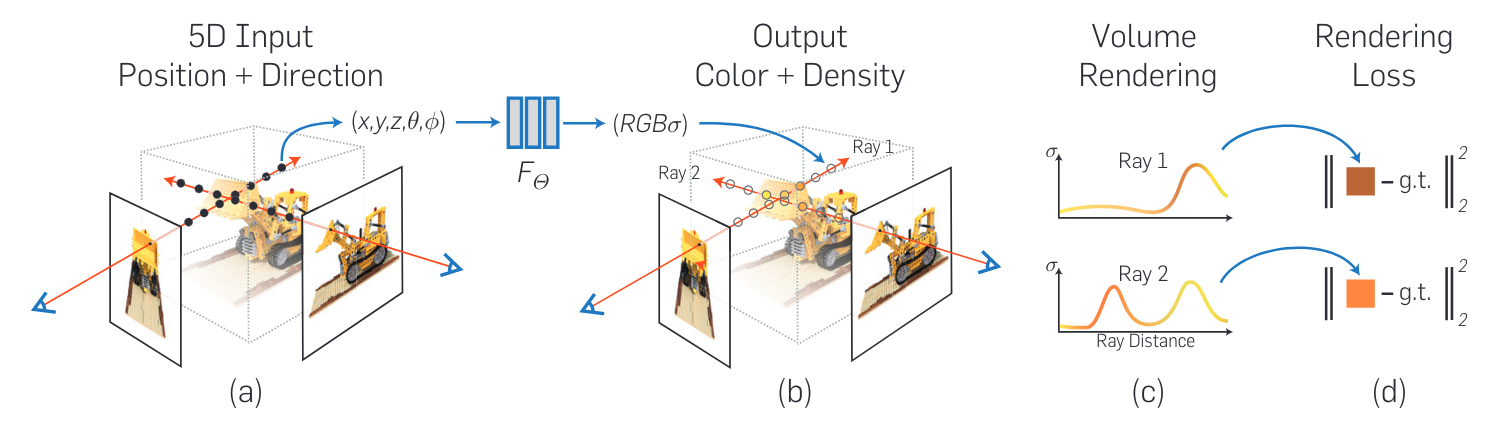
\includegraphics[width=\textwidth]{figures/bg-nerf.png}
  \caption{Overview of the NeRF scene representation and rendering procedure, illustrating the stages of sampling, neural processing, and image composition.}
  \label{fig:nerf-overview}
\end{figure}

\paragraph{Advantages of NeRF}
Compared to the methodologies discussed above, NeRF presents several advantages. It surpasses the capabilities of mesh and voxel-based methods in rendering high-resolution details and handling intricate geometries and material properties. The continuous volumetric representation is not only capable of producing more photorealistic images but also remains highly efficient in memory usage. This efficiency facilitates handling complex real-world scenes without the prohibitive storage and computation costs associated with traditional 3D representations.

In conclusion, NeRF's innovative use of neural networks for scene representation sets a new standard for photorealistic view synthesis, delivering high-quality results that are both computationally efficient and visually impressive.

% !TEX root = ../main.tex
%
\chapter{Related Work}
\label{sec:related}

\section{Instant NGP}

Instant Neural Graphics Primitives (Instant NGP) \cite{muller_instant_2022}, developed by NVIDIA, utilizes a multiresolution hash encoding that simplifies models while maintaining high performance and quality.
Its graphical user interface (GUI) plays a crucial role in enhancing accessibility and functionality, making it an important advancement in neural graphics technology.

\cleanparagraph{Simplified User Interaction}
The user interface of Instant NGP facilitates training and visualization of NeRFs \fref{fig:instant-ngp}.
The user is able to interactively explore 3D scenes in real-time and adjust parameters in order to achieve the desired results.

\begin{figure}[h!]
  \centering
  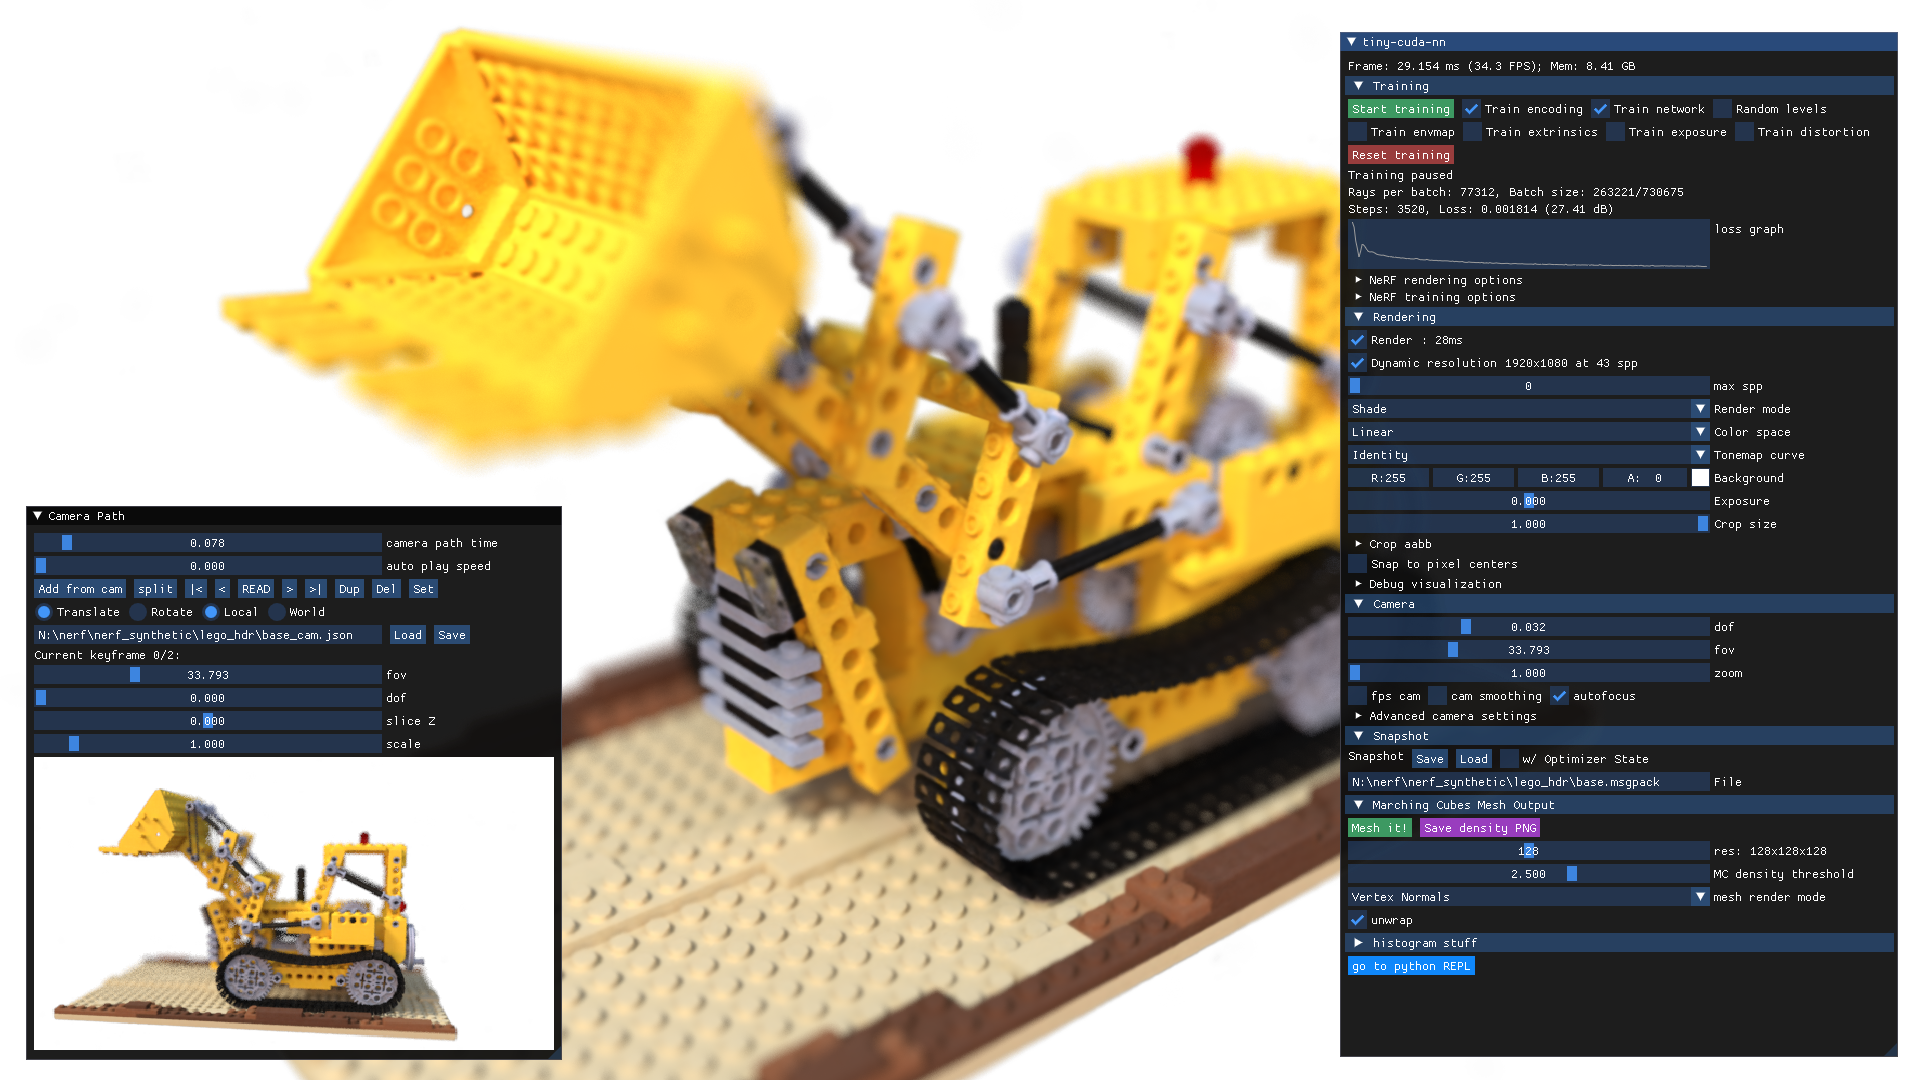
\includegraphics[width=\textwidth]{figures/realted-instant-ngp.png}
  \caption{Instant NGP's GUI rendering a NeRF scene, showing the 3D scene, camera path editor, and training parameters.
   \cite{muller_instant_2022}.}
  \label{fig:instant-ngp}
\end{figure}

\cleanparagraph{VR Mode}
The virtual reality (VR) mode of Instant NGP enhances user interaction by enabling immersive exploration of 3D environments in real-time.
This feature is especially beneficial for professionals like architects and game developers, who can benefit from experiencing their virtual spaces as if they were real.

\cleanparagraph{Camera Path Editor}
Instant NGP's camera path editor allows users to intuitively create and adjust camera trajectories, enhancing the creation of animations.
This tool is essential to professionals in visualization and animation, providing precise control over camera movements for detailed and smooth outputs.

\cleanparagraph{Limitations}
Despite advancements, Instant NGP's technical complexity and reliance on command-line interfaces for key operations remain significant barriers.
These aspects limit its accessibility to those with specific technical skills and deter broader creative applications.
The user experience still requires technical expertise, underscoring the need for more intuitive interfaces that simplify interaction and expand the user base beyond that of technical specialists.

\section{Nerfstudio}
\label{sec:related:nerfstudio}

Nerfstudio \cite{tancik_nerfstudio_2023} represents a significant advance in the accessibility of Neural Radiance Fields to non-technical users.
Its design focuses on modularity, ease of use, and integration capabilities, which are crucial for practical applications and academic research.

\cleanparagraph{Modularity}
Nerfstudio is built on a modular framework that allows users to easily customize and extend their NeRF implementations.
This modularity enables the use of a variety of input data formats, making it versatile for different real-world scenarios and setting it apart from Instant NGP.
A wide range of existing methods are already well integrated into Nerfstudio, including Instant-GPT \cite{muller_instant_2022}, their own Nerfacto \cite{noauthor_nerfacto_nodate} method that combines various existing techniques, and several of the previously mentioned extensions \cite{haque_instruct-nerf2nerf_2023,jan-niklas_dihlmann_signerf_2024}.

\cleanparagraph{Real-Time Web Viewer}
One of the standout features of Nerfstudio is its real-time web viewer, which enables visualization of NeRF training progress and outputs directly through a web browser \fref{fig:nerfstudio-viewer}.
This eliminates the need for high-end local GPU setups, such as in the case of Instant NGP, through remote sessions, broadening the tool's accessibility \cite{noauthor_nerfstudio-projectviser_2024}.

\begin{figure}[h!]
  \centering
  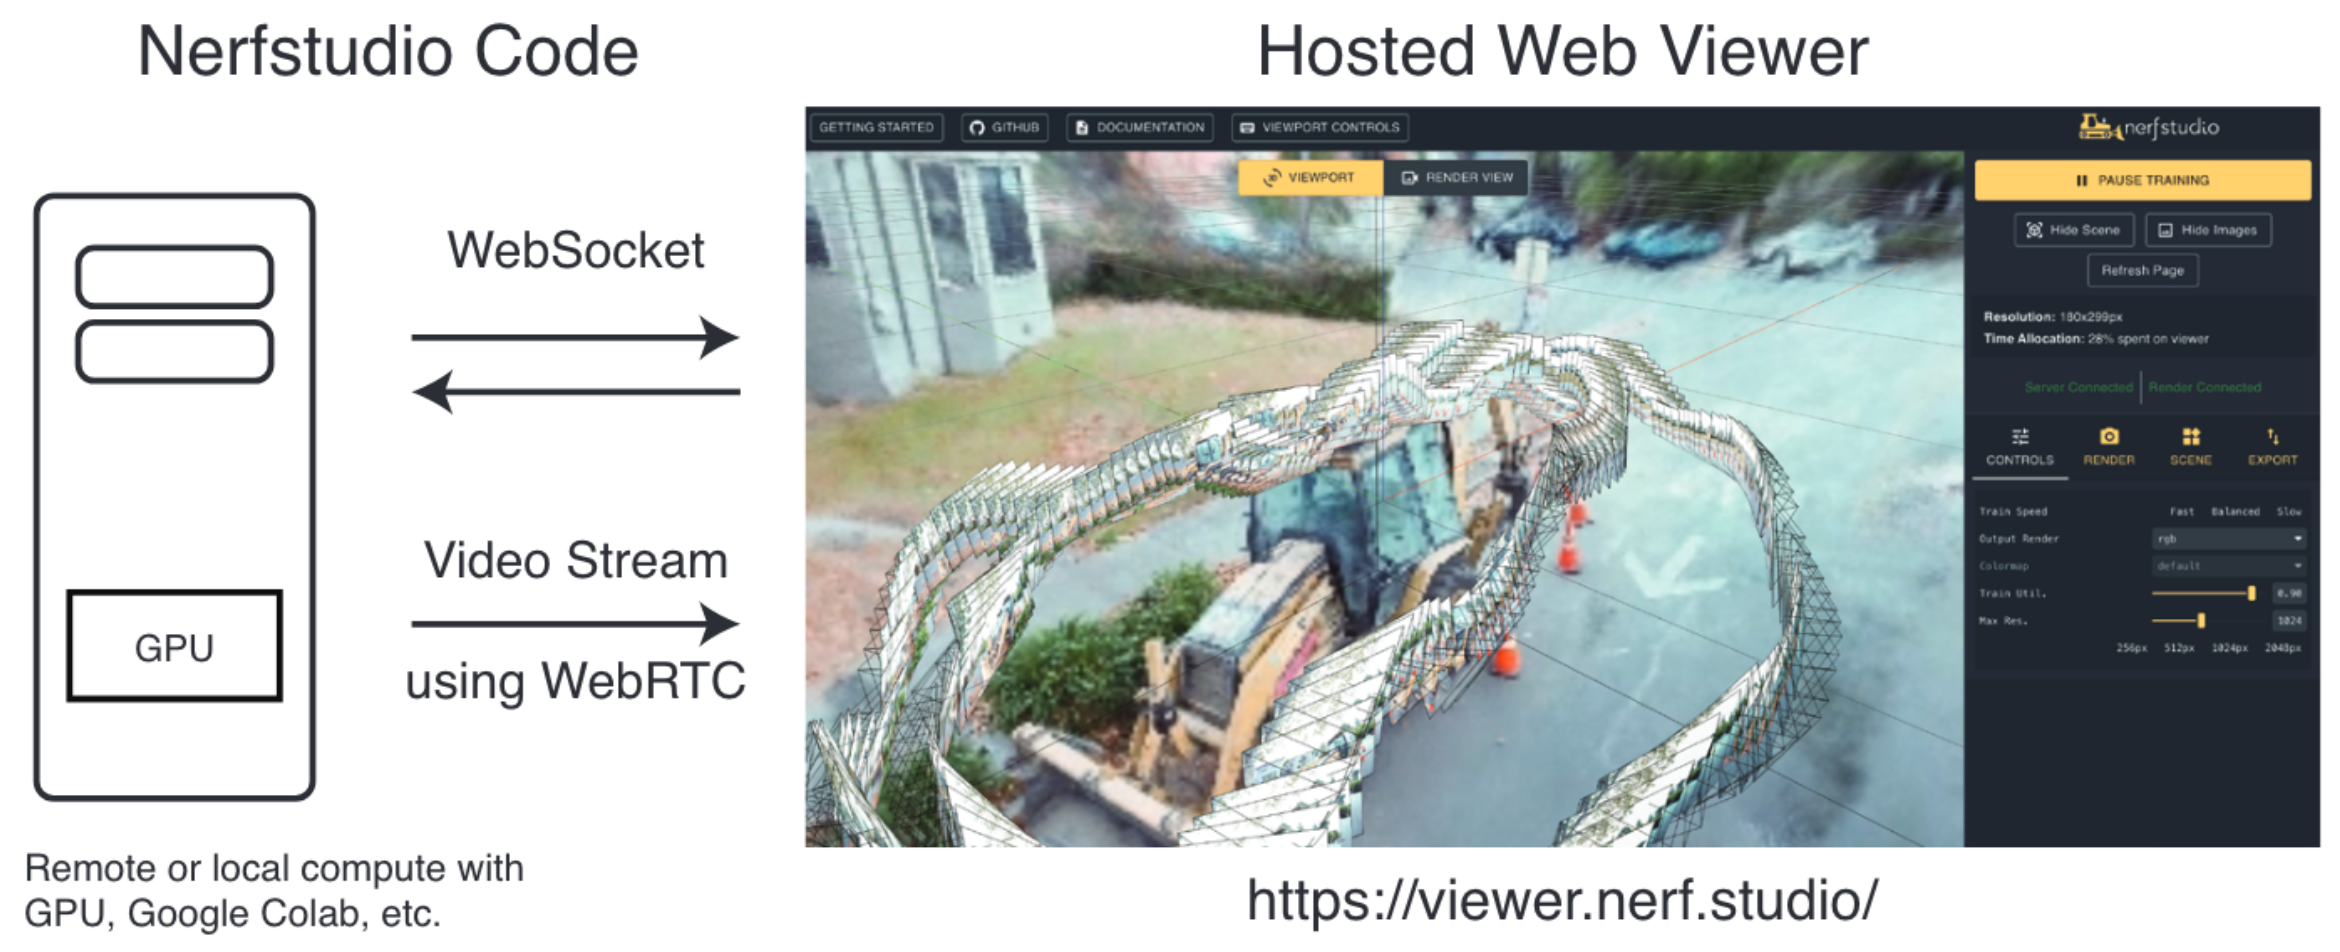
\includegraphics[width=\textwidth]{figures/related-nerfstudio-viewer.png}
  \caption{Nerfstudio's web viewer connected to a remote server running the training \cite{tancik_nerfstudio_2023}.}
  \label{fig:nerfstudio-viewer}
\end{figure}

\cleanparagraph{Flexibility of Data Handling}
Nerfstudio simplifies importing and exporting data, supporting a wide range of formats to accommodate various use cases.
Users can easily import images and videos, including data from mobile capture apps such as Polycam \cite{noauthor_polycam_nodate} and Record3D \cite{noauthor_record3d_nodate}.
Additionally, the framework supports exporting results in various formats such as videos, point clouds, and meshes.
This flexibility allows users to integrate NeRF outputs into diverse creative and technical applications.

\cleanparagraph{Community and Open-Source Contribution}
As an open-source project, Nerfstudio encourages community-driven development and continuous improvement, facilitating updates that keep pace with the latest research and technological advances.
This openness also allows users to adapt the tool to their specific needs.

\cleanparagraph{Limitations}
Nerfstudio is a welcome advancement improving on much of the features of Instant NGP.
However, it still requires a certain level of technical knowledge to operate effectively, limiting accessibility to non-technical users.
The tool's primary interactions are still command-line based, which presents a barrier to users who may prefer more intuitive graphical interfaces.

\section{Luma AI}
\label{sec:related:luma}

Luma AI \cite{noauthor_luma_nodate} is making Neural Radiance Fields accessible to non-technical users in a commercial space.
This platform leverages augmented reality (AR) to guide users through the capture process, greatly simplifying the creation of NeRFs from everyday smartphones.

\cleanparagraph{Guided Capture Process}
Luma AI utilizes AR to assist users in capturing images from optimal angles and distances, ensuring that the collected data is suitable for NeRF generation.
This guided process reduces the complexities involved in capturing the necessary footage for effective and streamlined NeRF creation.

\cleanparagraph{Cloud-Based NeRF Generation}
Once the footage is captured, it is automatically processed in Luma AI’s cloud-based system to generate a NeRF, requiring no user input for configuration.
This automation not only simplifies the user experience but also makes powerful 3D reconstruction technology readily accessible to a broad audience.

\cleanparagraph{Viewing and Editing}
Created scenes can be viewed directly within the app or through a web browser \fref{fig:luma-viewer}. 
While the editing capabilities are limited, users can make basic adjustments, reshoot parts of the scene, and interact with the generated NeRF in an intuitive manner.
The features here are similar to those offered in Nerfstudio's viewer, but with a more modern user-interface.

\begin{figure}[h!]
  \centering
  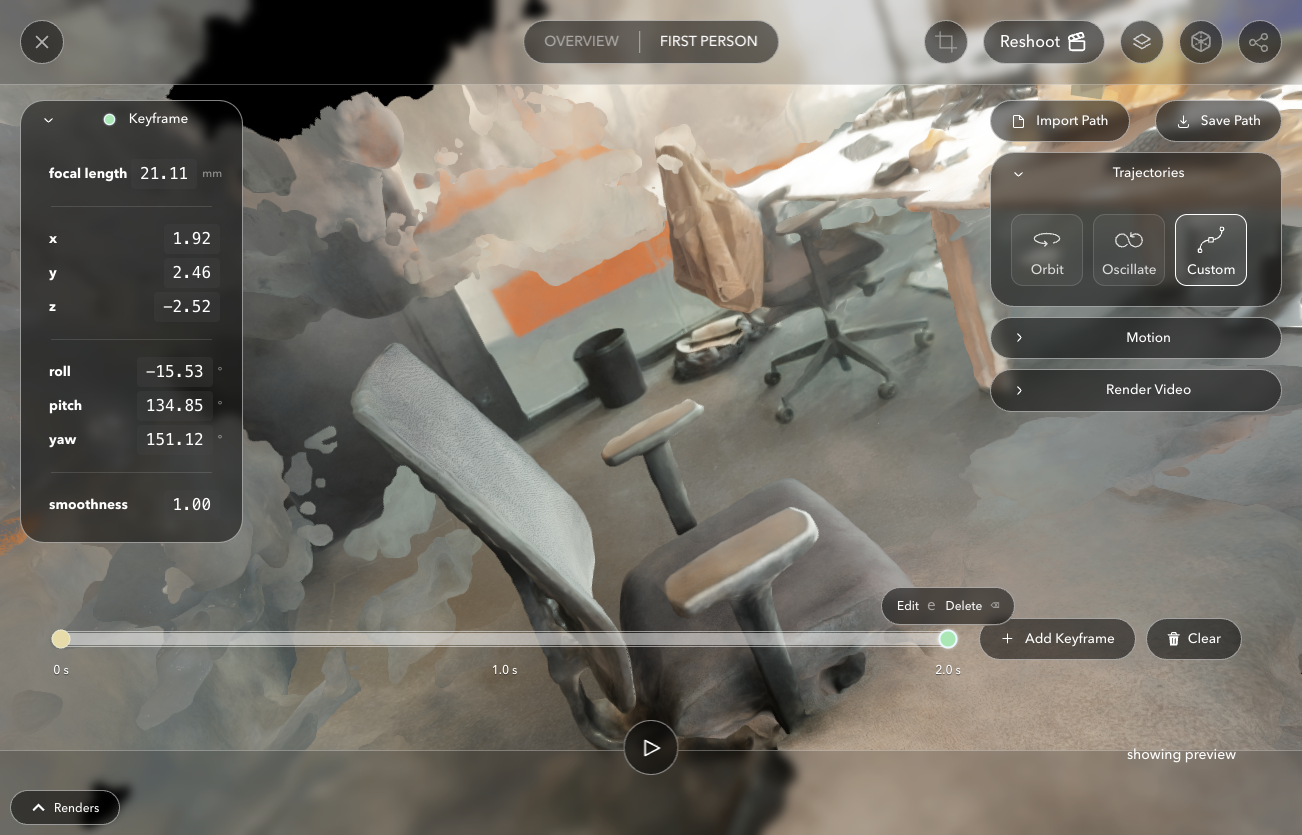
\includegraphics[width=\textwidth]{figures/related-luma.png}
  \caption{Luma AI Web Viewer in the camera path editor.}
  \label{fig:luma-viewer}
\end{figure}

\cleanparagraph{Export Capabilities}
Luma AI offers a variety of export formats for the generated scenes, allowing users to utilize these outputs in different applications or platforms, enhancing the utility of the captured NeRFs.
Additionally, they provide a social platform for the sharing and viewing of NeRFs, fostering a community of users around the technology.

\cleanparagraph{Limitations}
Despite its innovative approach, Luma AI's primary limitation lies in the lack of user control over the NeRF training process.
The automated system is designed to be user-friendly, yet it lacks the capacity to permit adjustments to the training parameters or the refinement of the final model.
This lack of control can result in suboptimal NeRF outputs for users who may require more precise or customized 3D representations.
Additionally, the proprietary nature of Luma AI may be a concern for users who prefer the flexibility and transparency offered by open-source solutions, as it limits the ability to understand and modify the underlying processes.

\section{Volinga Suite}

The Volinga Suite \cite{noauthor_volinga_nodate} aims to integrate Neural Radiance Fields into professional workflows.
It facilitates the adoption of NeRF by leveraging familiar platforms, thereby broadening the accessibility of NeRF to a wider range of users.

\cleanparagraph{Unreal Engine Integration}
Volinga's integration as a plugin for Unreal Engine \cite{noauthor_unreal_nodate} is a core feature that allows users to adopt NeRF seamlessly into existing pipelines \fref{fig:volinga-viewer}.
This integration is valuable for professionals already familiar with Unreal Engine, as it enables them to utilize advanced NeRF functionalities without additional training or significant adjustments to their current workflows.

\begin{figure}[h!]
  \centering
  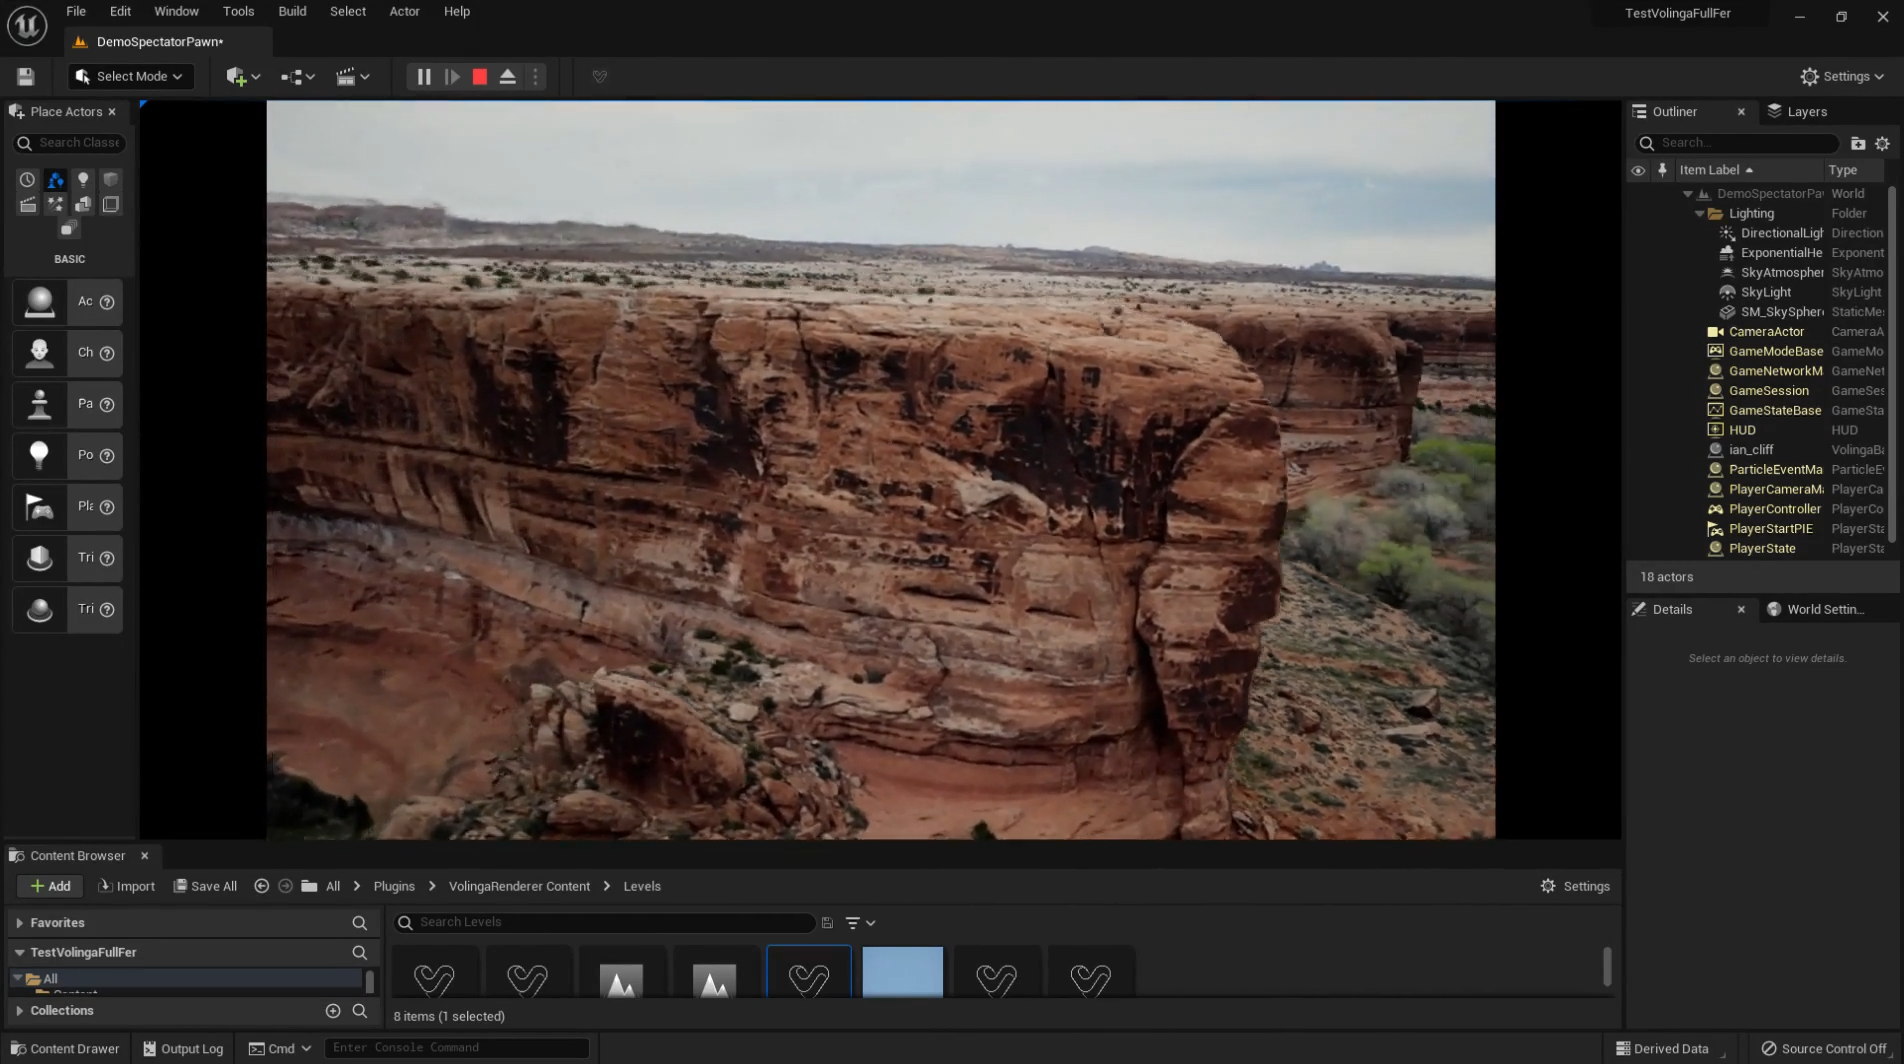
\includegraphics[width=\textwidth]{figures/related-volinga.png}
  \caption{Volinga Suite's integrated viewer in Unreal Engine \cite{noauthor_volinga_nodate}.}
  \label{fig:volinga-viewer}
\end{figure}

\cleanparagraph{Enhanced Control Over Training}
Volinga distinguishes itself from LumaAI by offering enhanced control over the NeRF training process.
Users have the ability to locally adjust numerous parameters, which enables precise tuning of the model's performance to meet specific project requirements.
This level of control is beneficial for projects where the quality of the NeRF output is critical.

\cleanparagraph{Local and Remote Training Capabilities}
The Volinga Creator component supports both local and remote training of NeRF models.
While remote training offers convenience and ease of access, local training provides advanced users with extensive configuration options and the ability to leverage powerful hardware, thereby maximizing the potential of NeRF technology under various usage scenarios.

\cleanparagraph{Limitations}
Volinga Suite's reliance on Unreal Engine for its integrated viewer may limit users who are unfamiliar with or do not wish to use this specific platform.
The web based viewer of Nerfstudio and Luma AI is more accessible in this regard.
Although Volinga is actively contributing to the open-source project Nerfstudio, its proprietary nature may also deter users or organizations that prefer open-source solutions.
   % INCLUDE: related work
% !TEX root = ../main.tex
%
\chapter{Methodology}
\label{sec:methodology}

This research was organized into three sequential phases: initial user research, prototype development, and user testing. 
Each phase was designed to inform and refine the subsequent stages, ensuring a systematic approach to developing a user-friendly NeRF interface. 
This iterative process aimed to align closely with user needs and feedback, fostering a design that is both intuitive and functional.

\section{Initial User Research}
\label{sec:methodology:user-research}

The foundational stage of this research involved conducting a series of in-depth interviews to gather insights into the user experience of NeRF technology. 
The primary objective is to understand the varied challenges, needs, and preferences of users, ranging from novices to experts in NeRF model creation, particularly those with ties to the film industry. 
This exploratory phase is crucial for identifying the key features and improvements necessary for a more accessible and efficient NeRF interface. (see Chapter~\ref{sec:user-research})

\section{Design and Development Process}
\label{sec:methodology:design-development}

The transition from initial user research findings to a functional prototype was a multi-step process focused on capturing user needs and translating them into a tangible design. 
This phase involved the creation of a user flow diagram, site map, wireframes, and a working prototype, each building upon the insights gained from the previous stage. (see Section~\ref{sec:design:ux})

\section{User Study and Evaluation}
\label{sec:methodology:study}

To evaluate the usability and overall utility of the developed NeRF interface prototype, a comprehensive user study was conducted. 
The primary aim of this study was to collect feedback on the prototype's user experience, identify any usability challenges participants encountered, and understand their satisfaction levels with the interface. 
Employing a mixed-methods approach allowed for a blend of quantitative and qualitative data collection and analysis, offering a multifaceted view of the prototype's performance in real-world tasks. (see Chapter~\ref{sec:study})       % INCLUDE: concepts
% !TEX root = ../main.tex
%
\chapter{User Research}
\label{sec:user-research}

\section{Participant Selection Criteria}
\label{sec:user-research:criteria}

Participants were selected with care, taking into account their previous experience with NeRF technology and their connection to the film industry. 
This resulted in a group of four experts. 
The selection of participants ensured a diversity of perspectives, encompassing a broad spectrum of technical proficiency and practical applications of NeRF. 
The study aimed to uncover both the shared challenges faced by all users and the unique requirements of distinct user groups within the film industry by including individuals who have utilized NeRF in various capacities.

\section{Interview Methodology}
\label{sec:user-research:interview}

The interviews were designed as semi-structured conversations, following a core set of prepared questions (see Appendix \ref{sec:appendix:interview-questions}).
However they also allowed for spontaneous discussions and additional queries. 
The interviews were conducted in a one-on-one format (three online, one in person), facilitating a personalized dialogue with each participant. This approach allowed for the collection of insights into individual experiences and perspectives. 
Although the interviews were prepared in English, all conversations were held in German to ensure comfort and clarity for participants, potentially leading to more candid and informative discussions.

The structured flow of questions began with learning about the participants' backgrounds and experiences with NeRF technology, gradually moving towards more detailed questions about their specific needs, challenges, and desired improvements in NeRF interfaces. 
Additionally, participants were encouraged to suggest potential enhancements to the NeRF interface that they believed would enhance its usability and effectiveness for their professional or academic projects.

To ensure comprehensive analysis, interviews were recorded and transcribed with the participants' consent, allowing for a detailed review and coding of the responses. 
This process enabled the identification of recurring themes, challenges, and preferences across the participant group, providing a solid foundation for the subsequent phases of prototype development and user testing. 
The insights gained from this initial research phase were instrumental in shaping the direction and focus of the interface design, ensuring that it would effectively address the real-world needs of NeRF users.

\section{Key Findings}
\label{sec:user-research:findings}


\cleanparagraph{NeRF in the Film Industry}
NeRF technology is being explored for various applications in the film industry, including visual effects, virtual production, and pre-production location scouting. 
Despite its potential to simplify the creation of 3D scenes, current limitations in model quality, lack of editable models, and insufficient detail hinder its professional use. 
However, its capability for rapid 3D scene captures offers significant benefits for pre-visualization and planning in the pre-production phase, although concerns about model scale accuracy for export remain. 
\cite{P2, P4}

\cleanchapterquote{So in the planning phase I think [NeRF] was pretty well received, the set visit, the planning of the actual shoot, but the quality wasn't that convincing yet.\footnotemark}{Participant 4}{}
\footnotetext{Also in der Planungsphase kam [NeRF] glaube ich ziemlich gut an, Setbegehung, Planung vorne vom eigentlichen Dreh, aber die Qualität war halt noch nicht so überzeugend.}


\cleanparagraph{Optimizing Parameters and Workflow}
Creating NeRFs typically involves three main steps: pre-processing input data, training models, and exporting outputs. 
Technical users emphasize the importance of parameter optimization in improving NeRF quality, with iterative training and results analysis being crucial parts of their workflow.
Tools such as TensorBoard \cite{noauthor_tensorflowtensorboard_2024} are utilized for quantifying variations in training outcomes. 
\cite{P1, P3}

\cleanchapterquote{Problems? Optimization, i.e. data sets. In training, I would say a big thing is optimization and parameterization, especially in Nerfstudio.\footnotemark}{Participant 1}{}
\footnotetext{Probleme? Optimisierung, also Datensätze.
Beim Training würde ich sagen, eine gro{\ss}e Sache ist die Optimierung und die Parameterisierung, vor allem in Nerfstudio.}

\cleanparagraph{User Interface and Accessibility}
A consensus among users indicates a clear need for an intuitive, comprehensive user interface that minimizes reliance on console commands.
Features that allow users to visually navigate and control the NeRF creation pipeline, including real-time progress feedback and the ability to pause and adjust processes at any stage, are highly valued. 
\cite{P1, P2, P3}

\cleanchapterquote{The most important thing for me would be that I don't have to do anything in the console. In other words, that I can simply start the program and then do everything in the UI, upload it and then it will be executed somehow.\footnotemark}{Participant 2}{}
\footnotetext{Das Wichtigste wäre für mich, dass ich halt nichts in der Konsole machen muss. Also, dass ich einfach das Programm starte und dann alles in der UI machen kann, hochladen und dann auch irgendwie durchgeführt werde.}

\cleanparagraph{Comprehensive Error Handling and Visualization}
Effective error feedback and clear, informative visualization tools are critical for user satisfaction. 
Users have expressed frustration with vague error messages and cumbersome command-line interactions for troubleshooting and adjustments. 
\cite{P2, P3}

\cleanchapterquote{So if there is an error message, then it would be cool if they would somehow tell you more precisely what the error is, and not just any log.\footnotemark}{Participant 2}{}
\footnotetext{Also wenn eine Fehlermeldung ist, dann wäre es halt cool, wenn die einem das irgendwie genauer sagen würden, was der Fehler ist, und dann nicht einfach so irgendein Log.}

\cleanparagraph{File Management and Project Structure}
Efficient file and project management, with clear distinctions between different stages and support for various input formats, is essential. 
Users discuss challenges with current tools regarding data organization, suggesting improvements for handling input data and managing projects​​.
\cite{P1, P3}

\cleanparagraph{Integration and Export Options}
Strong integration capabilities with popular 3D and VFX software and flexible export options are desired. 
Users discuss the importance of being able to easily import NeRF-generated scenes into tools like Unreal Engine \cite{noauthor_unreal_nodate} or Blender \cite{noauthor_blender_nodate} for further processing and use in production-quality projects​​.
\cite{P1, P2, P4}

\cleanparagraph{Multi-Mode Operation}
The necessity for multi-mode operation in NeRF tool interfaces emerges as a significant insight, underscoring the importance of accommodating a broad spectrum of users, from novices to experts. 
A simplified mode is proposed to cater to beginners, offering an intuitive and streamlined workflow.
In contrast, an advanced mode is tailored for experienced users requiring detailed control over the NeRF creation process. 
\cite{P1, P2, P3, P4}

\cleanchapterquote{It just has to be understandable enough that film students aren't afraid of it. But still, not limit how much you adjust your parameters.\footnotemark}{Participant 1}{}
\footnotetext{Es muss halt verständlich genug sein, dass Filmstudenten davon keine Angst haben. Aber trotzdem, [das Ma{\ss}] wie sehr du deine Parameter ansetzen kannst [nicht] zu limitieren}

\subsection*{Summary}

These findings highlight the demand for a NeRF tool interface that is user-friendly, versatile, and capable of supporting a wide range of workflows and user expertise levels. 
The optimal tool would integrate intuitive project management and visualization features with robust customization options, effective error handling and feedback mechanisms, and efficient performance management capabilities.
% !TEX root = ../main.tex
%
\chapter{User Interface Design}
\label{sec:design}

This chapter outlines the design of the prototype, focusing in the user interface and the user experience. The design process was informed by the initial user research.

\section{User Flow and Navigation}
\label{sec:design:flow}

As an initial step in the design process, a user flow diagram was created to visualize required user interaction and their relations. 
In a first rough sketch, key interactions were arranged in a linear sequence, representing the typical workflow when creating NeRF models (\ref{fig:design:flow-1}).

\begin{figure}[htb]
	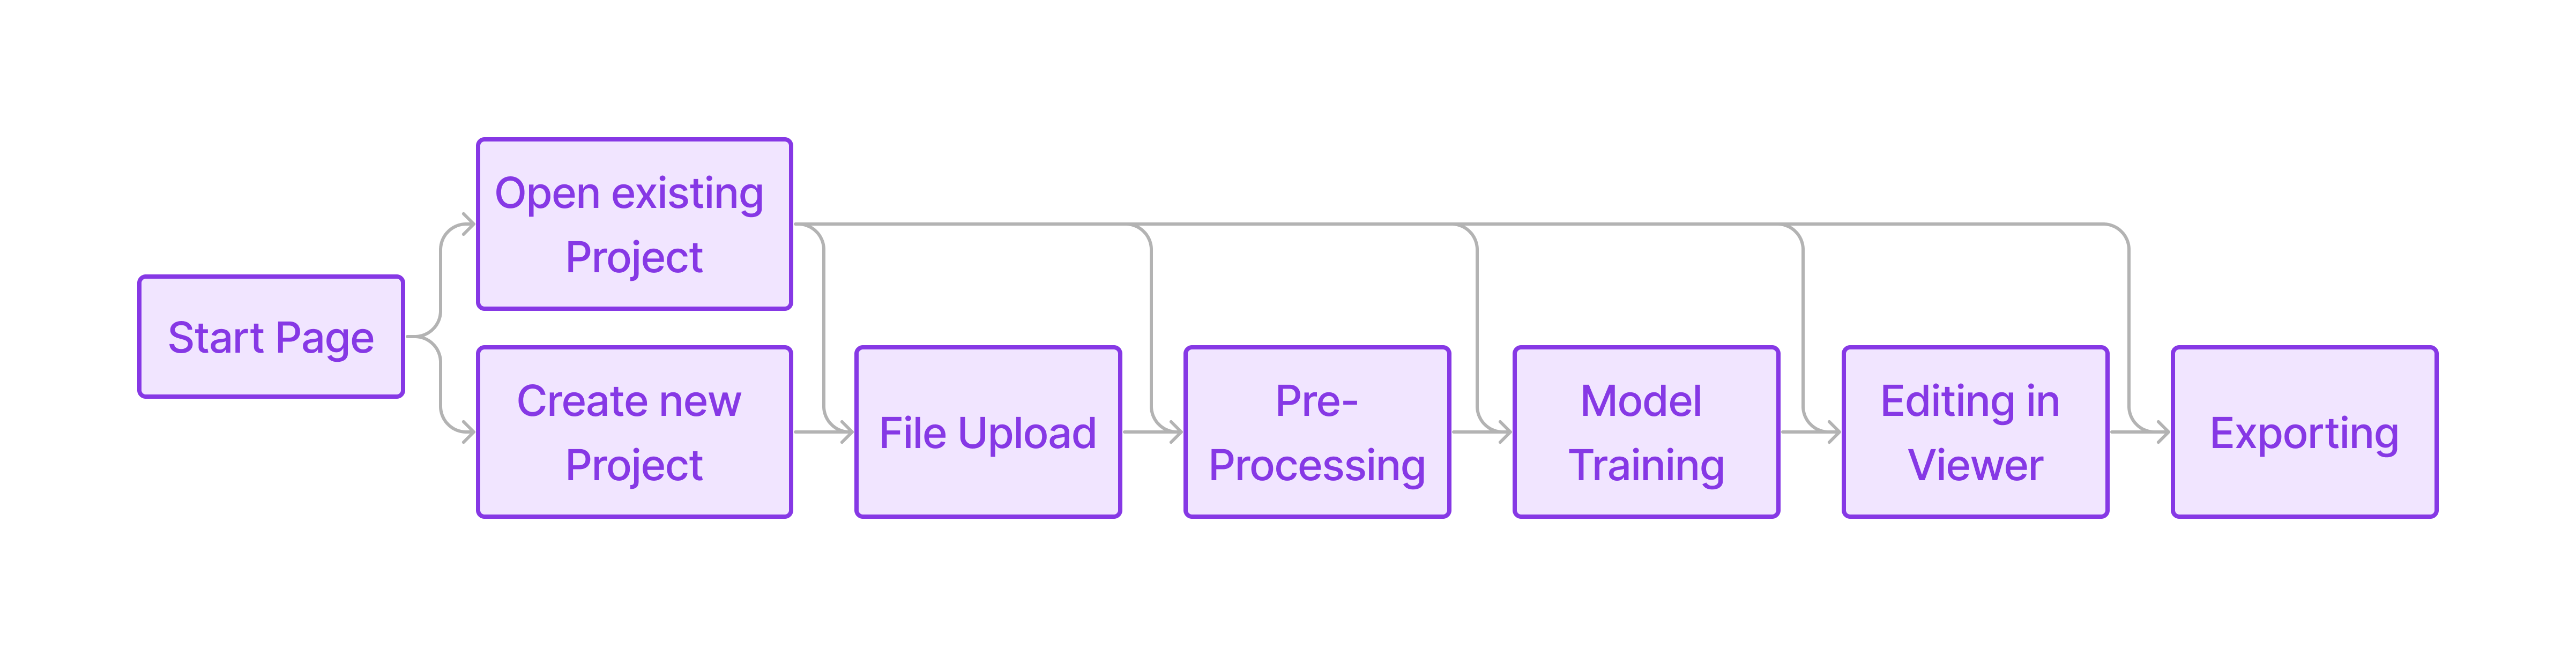
\includegraphics[width=\textwidth]{figures/flow-1.png}
	\caption{Flow Diagram}
	\label{fig:design:flow-1}
\end{figure}

Building on this outline, complex interaction were broken down into smaller steps to scope out what user actions were required to complete a task.
Interactions could then be group into views, and the navigation between these views could defined.
The views were also enriched with more detailed information on the exact user interactions (\ref{fig:design:flow-2}).

\begin{figure}[htb]
  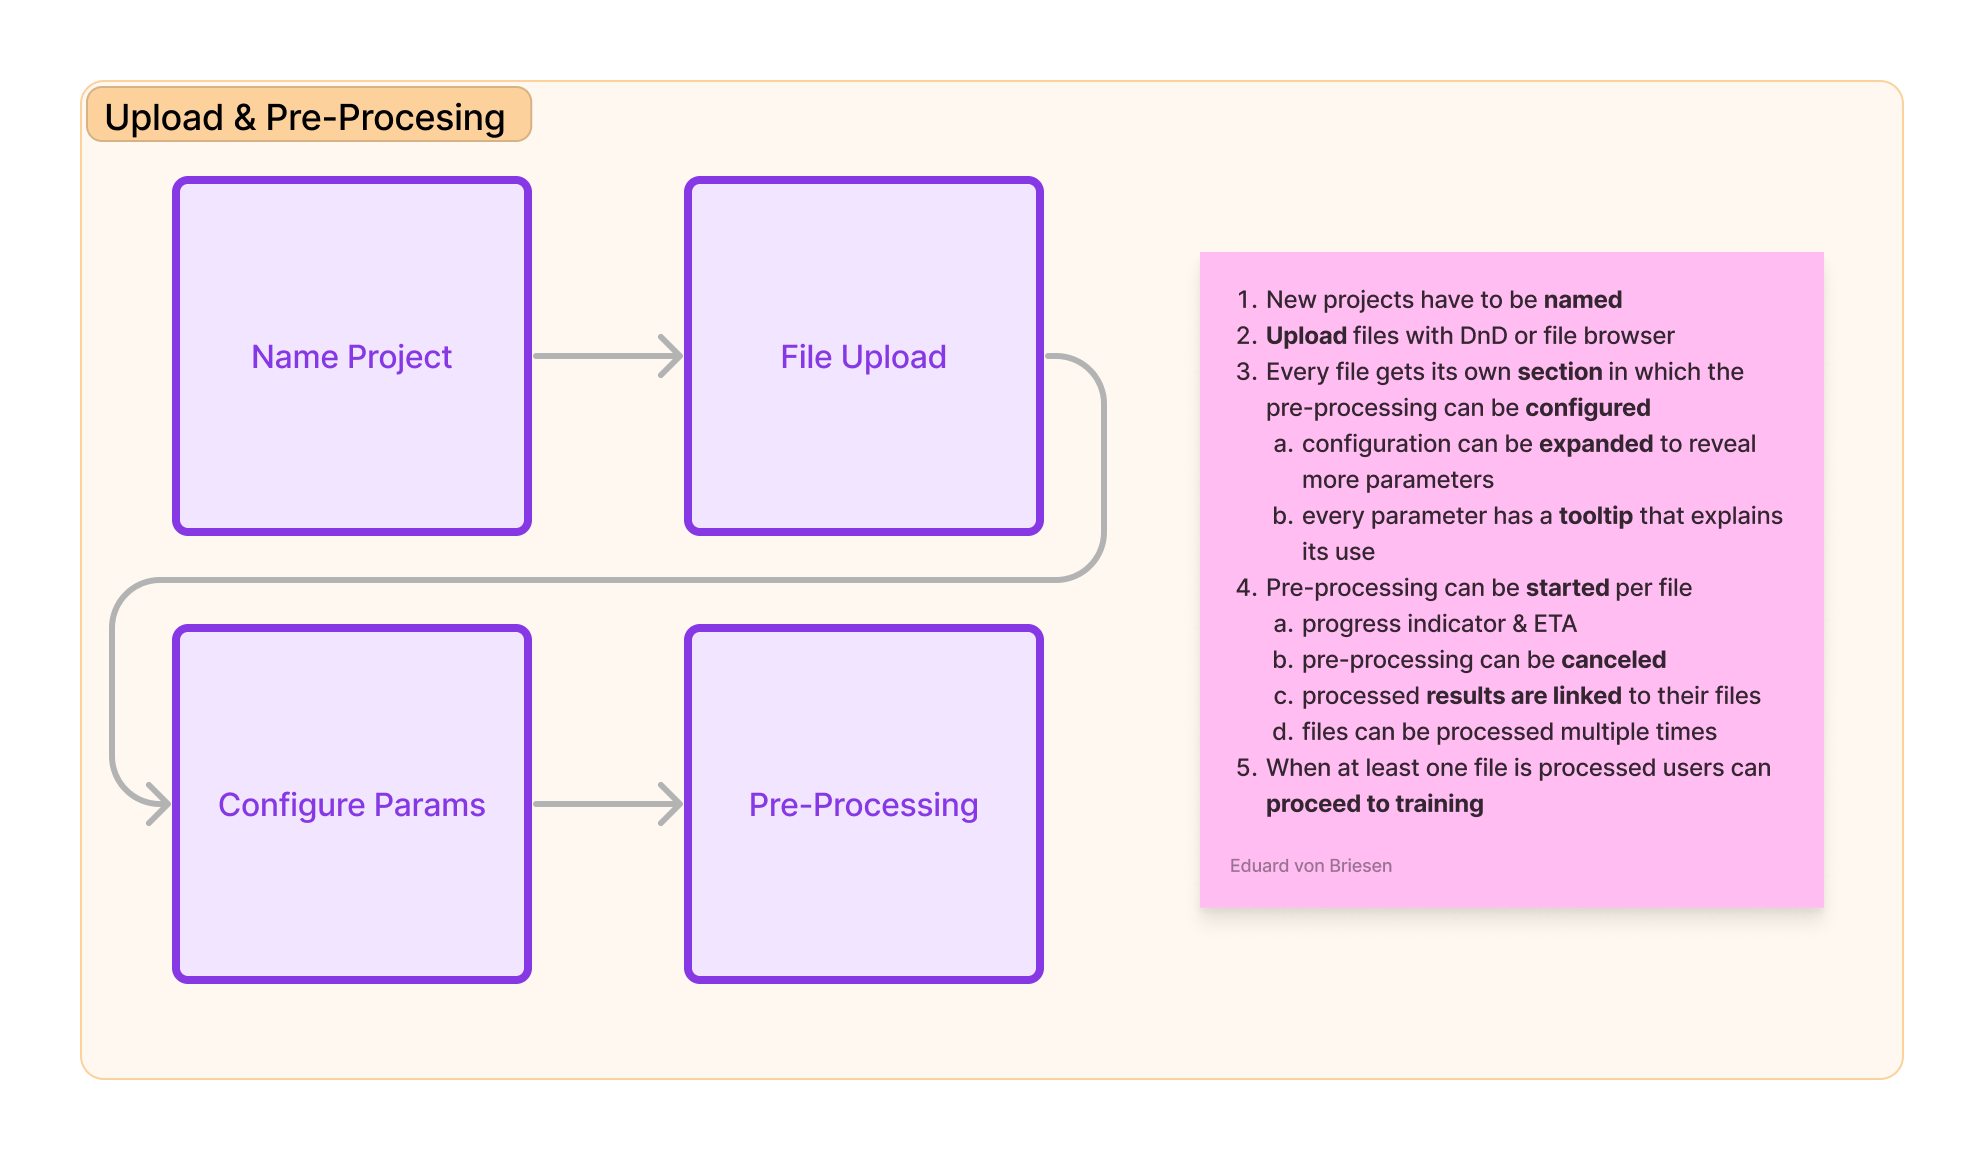
\includegraphics[width=\textwidth]{figures/flow-2.png}
  \caption{Excerpt of a View from the Flow Diagram with detailed interactions}
  \label{fig:design:flow-2}
\end{figure}

These diagrams were used as a reference throughout the design and development process, to ensure a structure that followed the user's mental model and to keep the user interface consistent.

\section{User Interface}

The user interface was designed to be as simple as possible, while still providing all necessary functionality. 
The design of the prototype can be broken down into two main parts: a dashboard that gives an overview of all projects and a project section that provides users with the tools to create and edit NeRF models.

\subsection*{Dashboard}

The dashboard is the first view that users see when opening the application. It shows all previously created projects and allows users to create new ones. 
Projects are represented as cards, showing the project name, a preview of on the provided input images (if present), and tags the indicate the current status of the project.
An additional card is present through which users can create a new project, by providing a name.
Projects can be opened by clicking a button on the respective card, when creating a new project, users are redirected to the project section.

\begin{figure}[htb]
  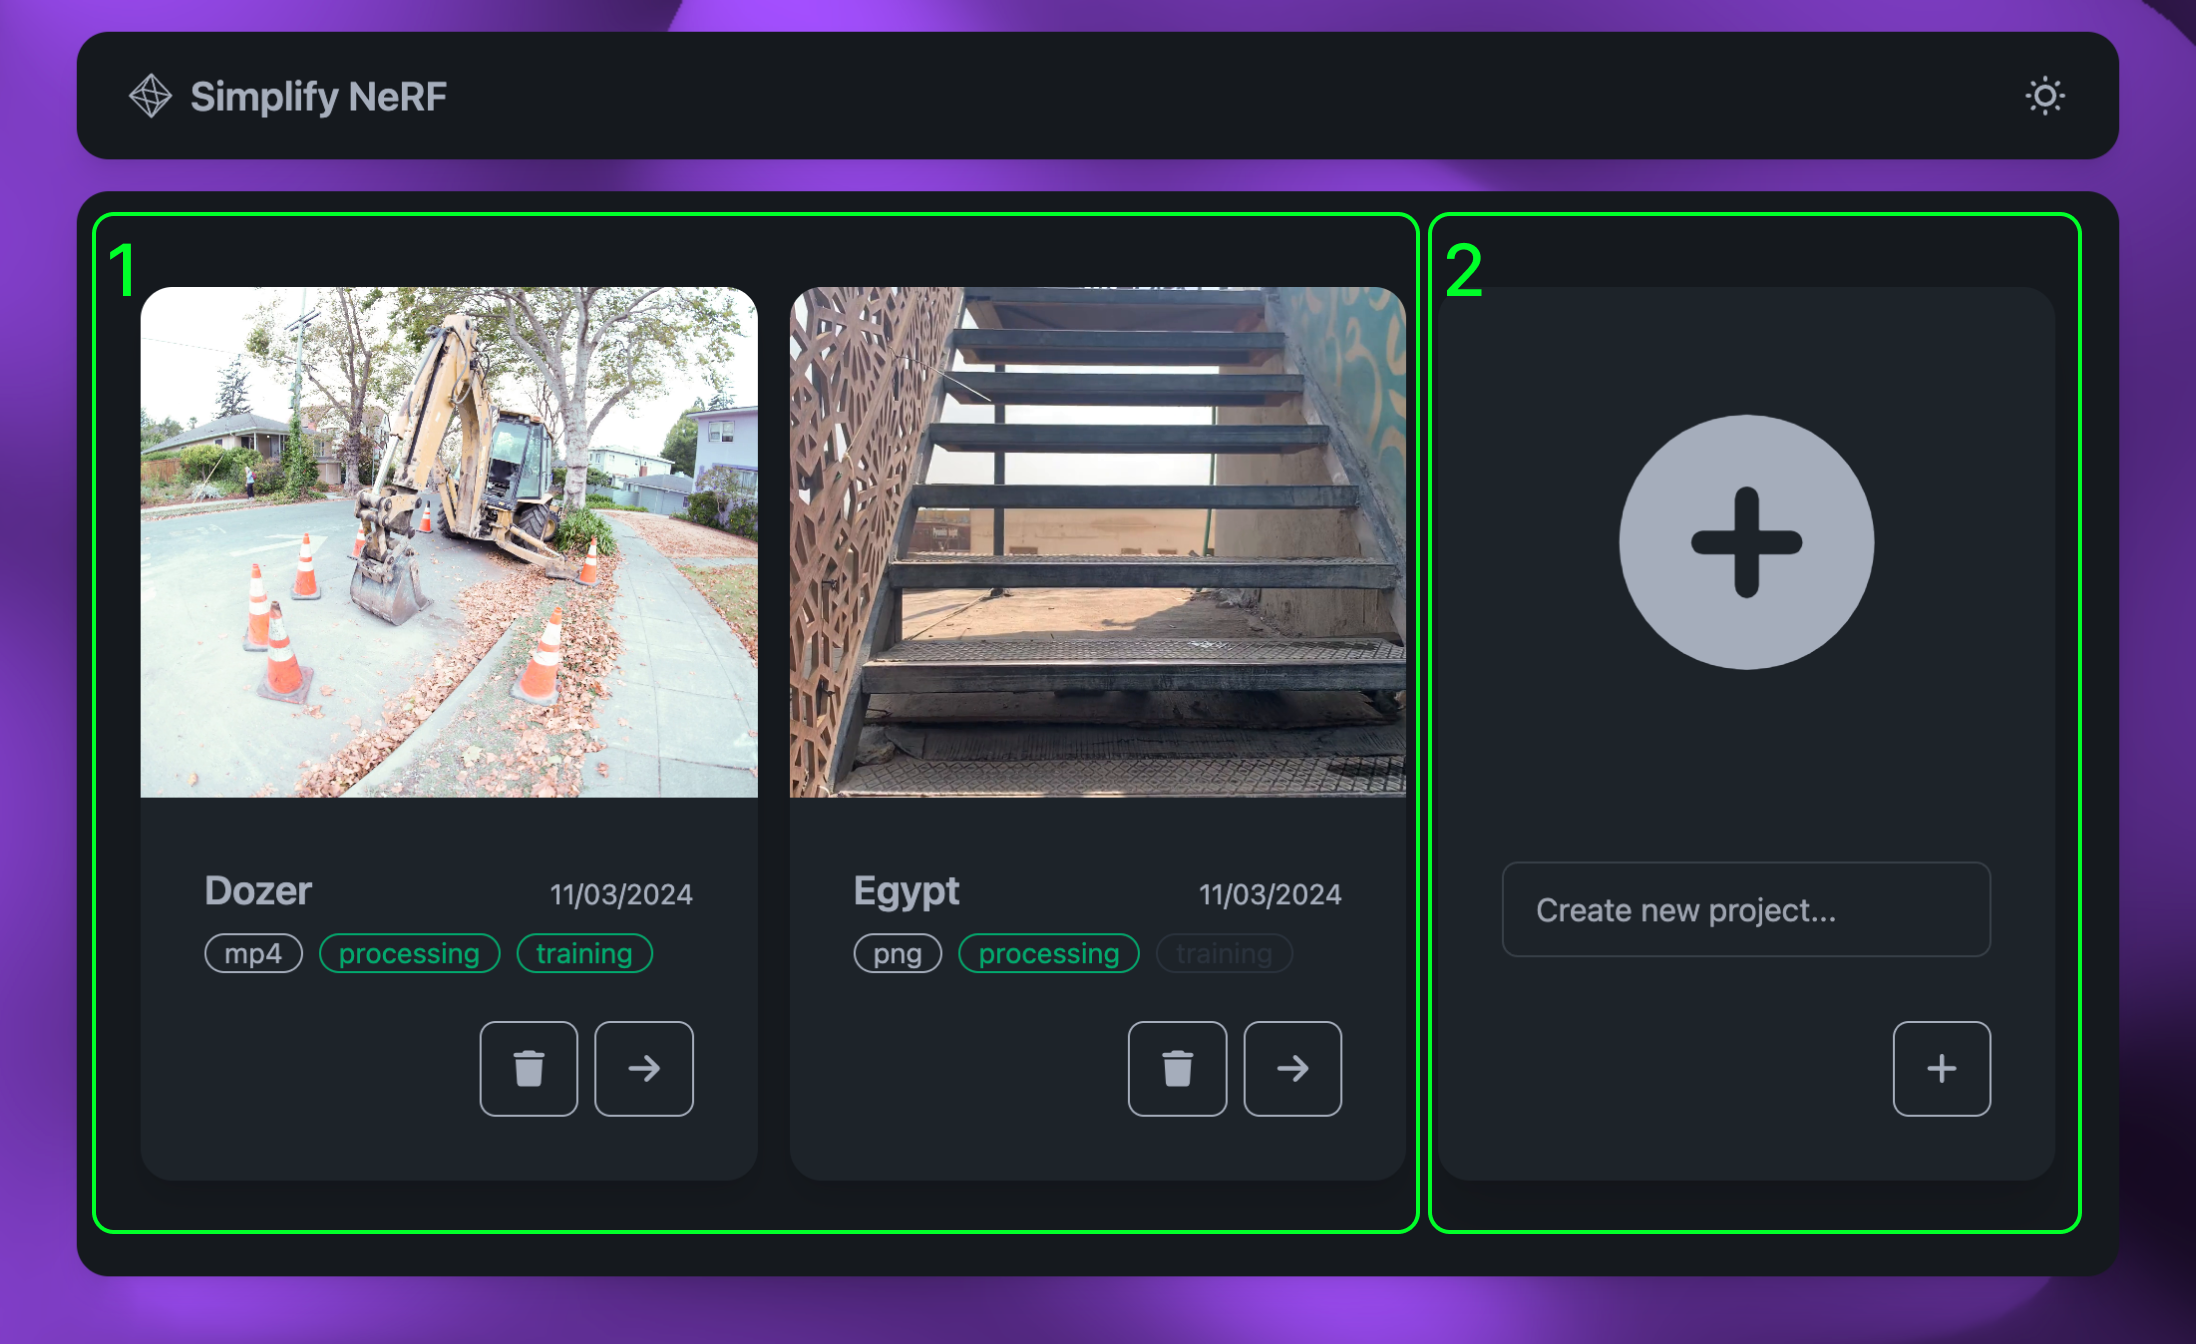
\includegraphics[width=\textwidth]{figures/view-overview.png}
  \caption{Dashboard}
  \label{fig:design:dashboard}
\end{figure}

\subsection*{Project Section}

The project section is the core of the application, through which users can create and edit NeRF models.
The section is divided into three parts: the input section, the training section, and the rendering section.
Across all sections, users user can track there progress through a progress bar at the top of the screen, that also enables easy navigation between the different sections.

\subsubsection{Input Section}

The input section combines the first few interactions, as mapped out in the user flow diagram.
First users are prompted to upload there input data, which can be done by dragging and dropping files into the browser window or by clicking a button to open a file dialog.
Files can be either a set of images or a video, and there are some guardrails in place to ensure that the input data is valid.
Once the input data is uploaded, it has to be processed before it can be used for training. 
The pre-processing can be configured by the user, this includes parameters such as the lense-type, or matching method.
Parameter input fields vary based on the type of input data, and are only shown when relevant.
Once the user is satisfied with the settings, they can start the pre-processing.
Feedback on the progress of the pre-processing is given through a console that shows the output of the process running on the server.
When the pre-processing is finished, the user can move on to the training section. 

\begin{figure}[htb]
  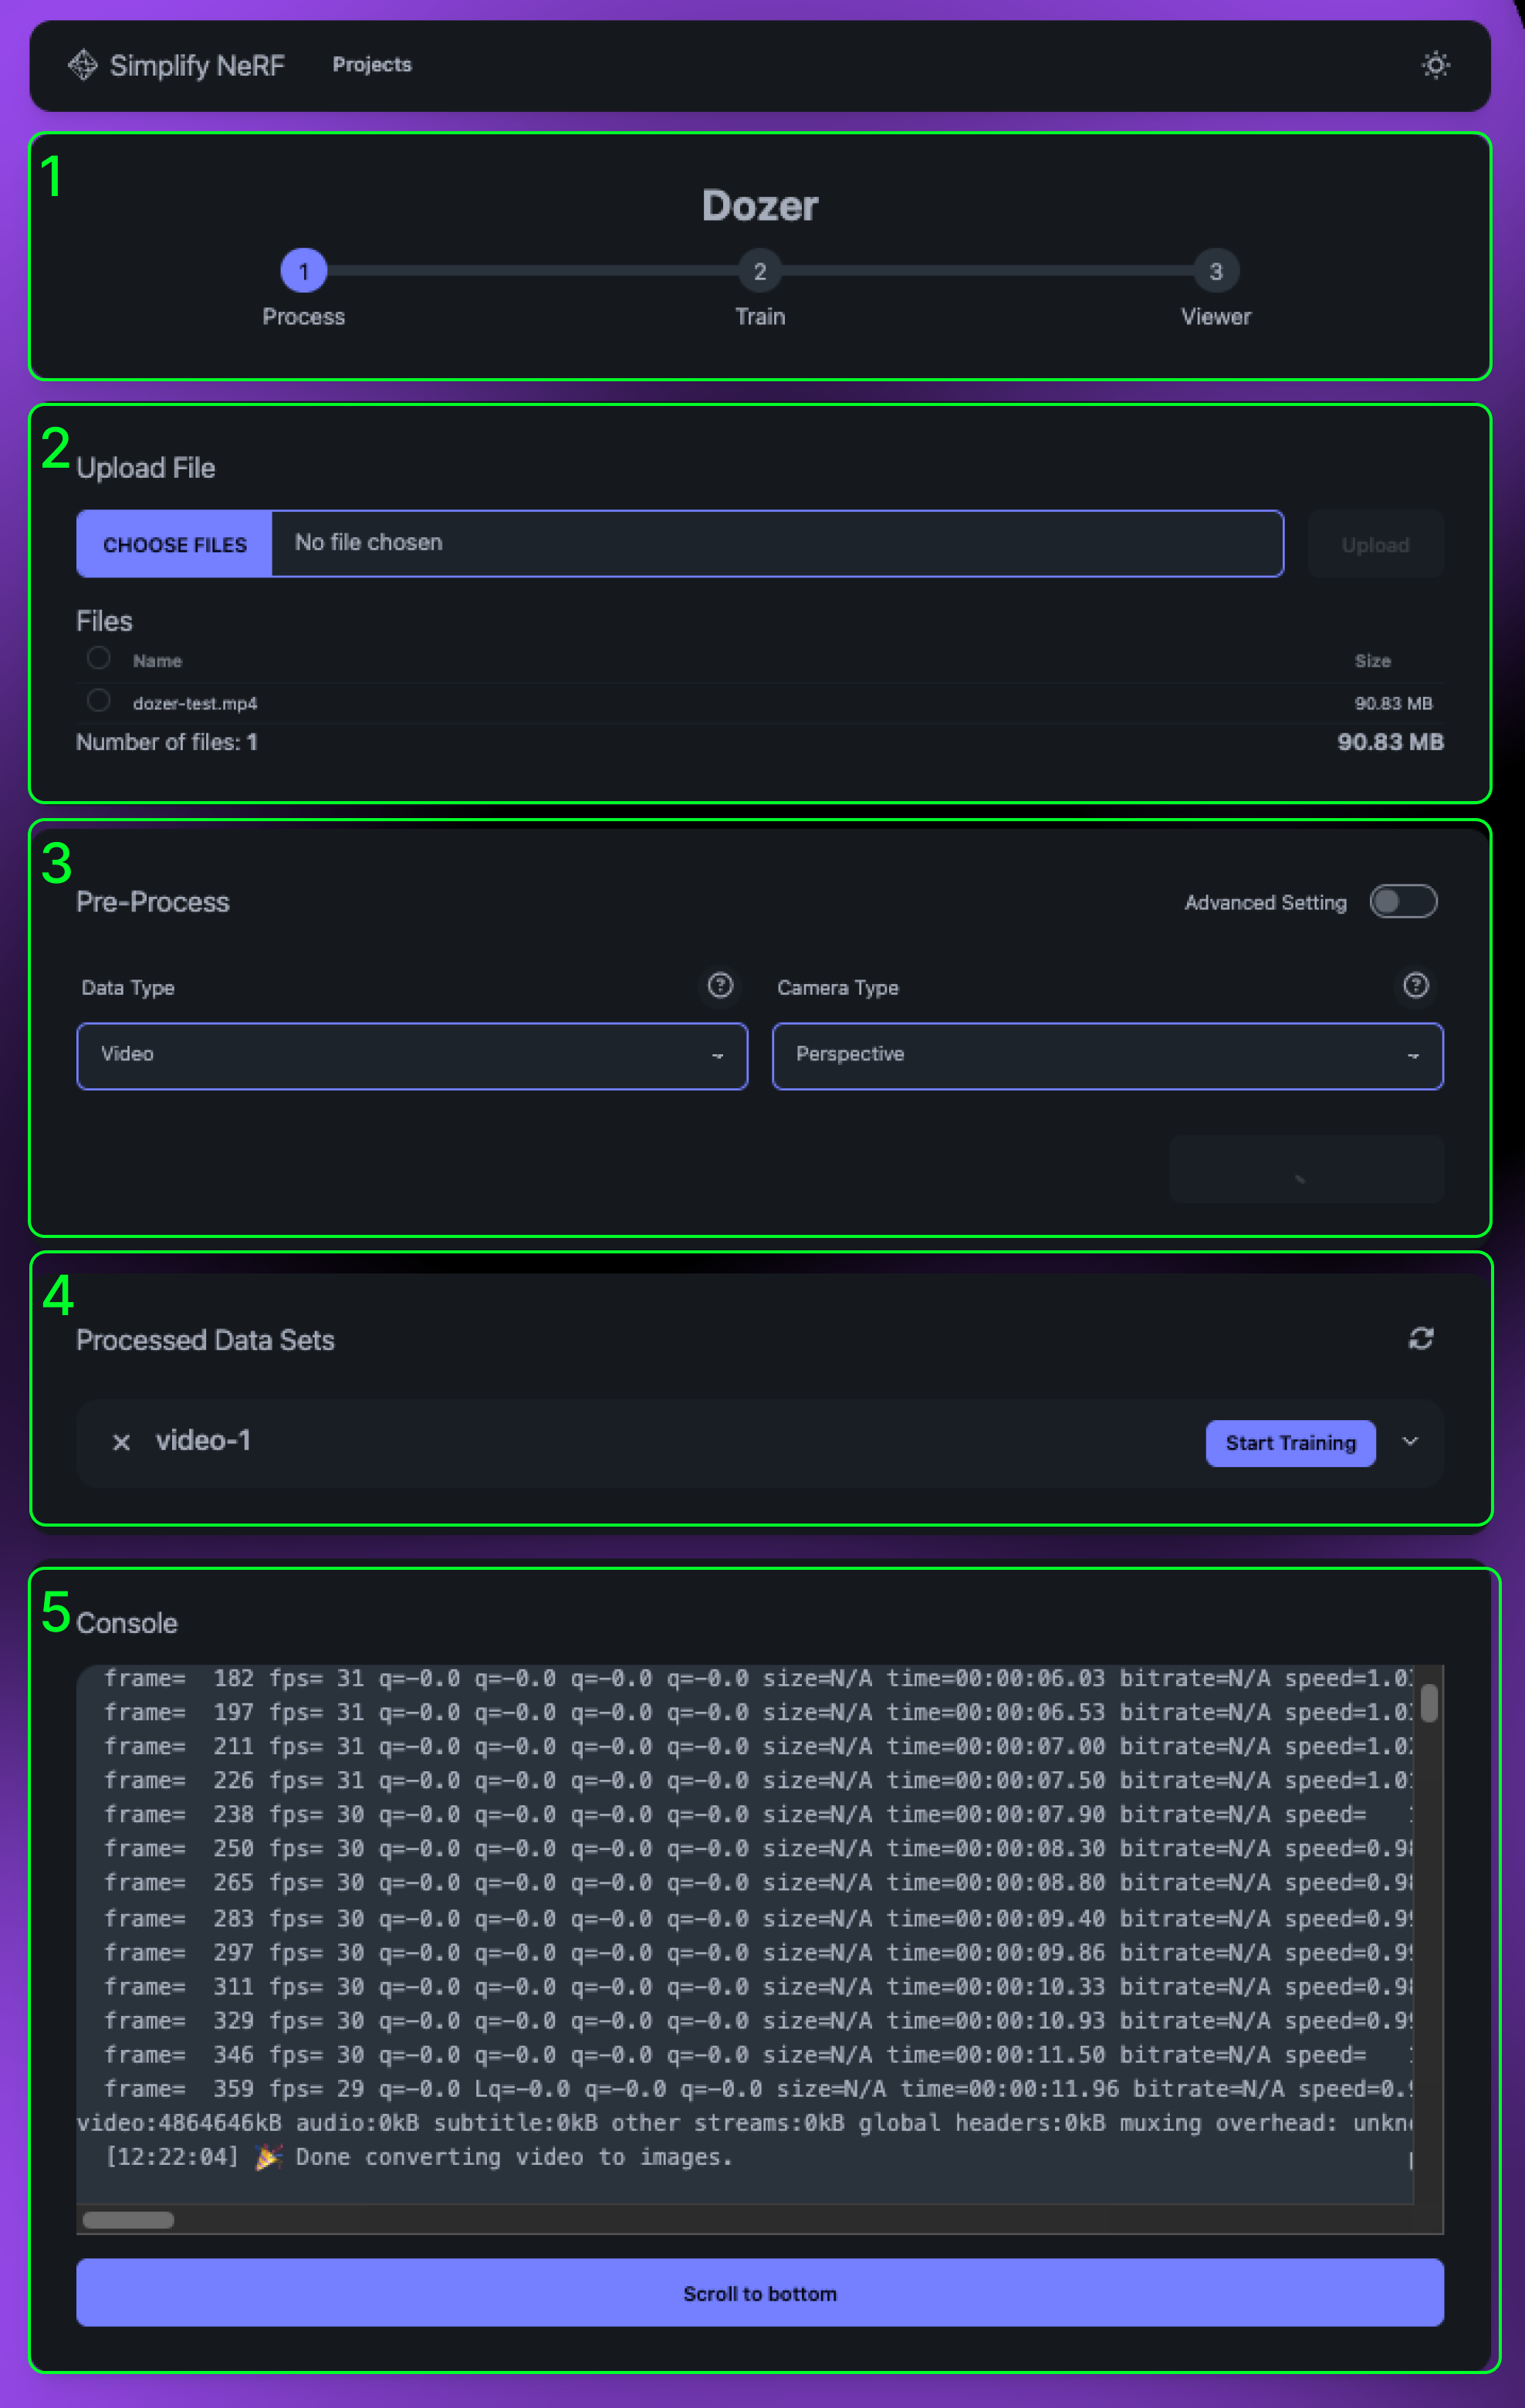
\includegraphics[width=\textwidth]{figures/view-process.png}
  \caption{Processing Input Data}
  \label{fig:design:input-section}
\end{figure}

In case the data was already pre-processed, a list ist visible that shows all available pre-processed data, and the user can select one to use for training.
Users can also inspect the configuration with which the data was pre-processed, and delete it if necessary.

\subsubsection{Training Section}

The training section is structured similarly to the input section, with a form that allows users to configure the training process, and a console that shows the output of the training process running on the server.
When the user is satisfied with the configuration, they can start the training process.

\begin{figure}[htb]
  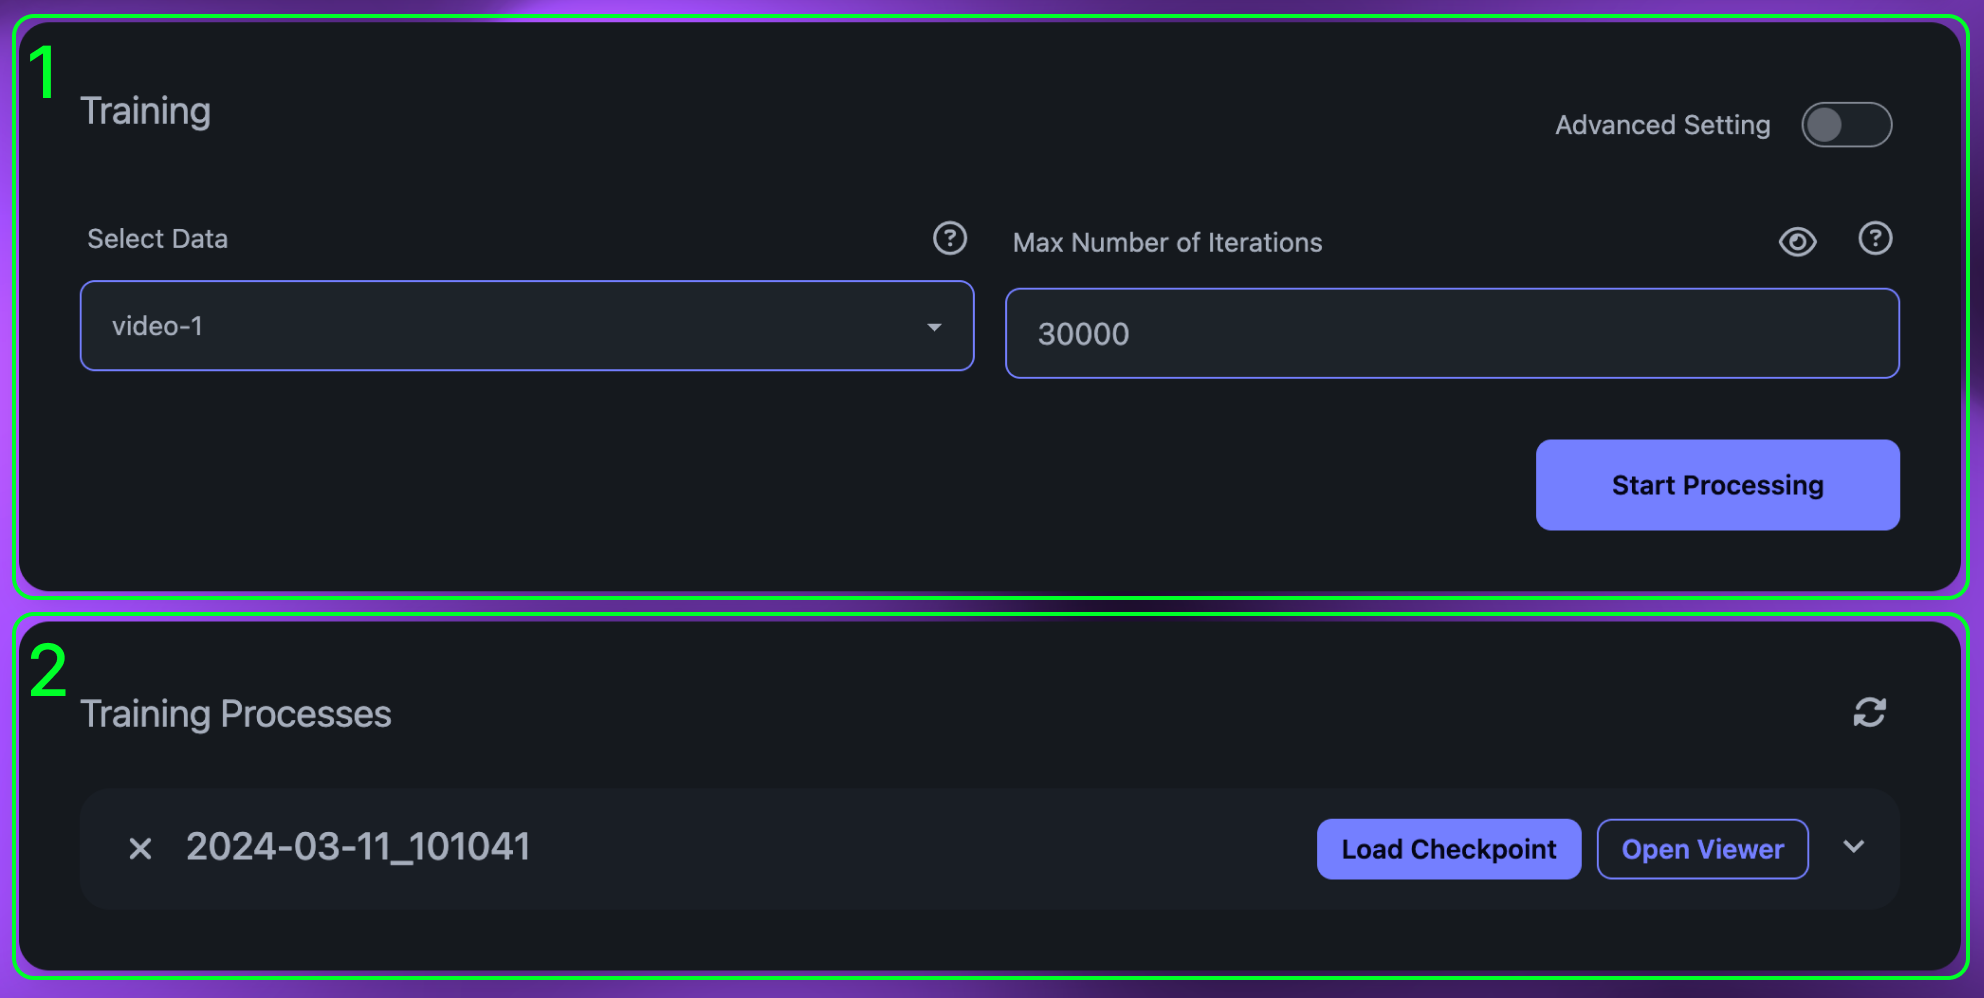
\includegraphics[width=\textwidth]{figures/view-train.png}
  \caption{Training Section}
  \label{fig:design:training-section}
\end{figure}


Previous training runs are listed, and users can inspect the configuration with which the training was run, and delete it if necessary. 
The viewer can be opened to inspect the results of the training run, or an existing checkpoint can be selected to continue training from that point.

\subsubsection{Viewer Section}

The viewer section is the final step in the process, and allows users to inspect there NeRF model, while it is still training or after the training has finished.
At its core is the Nerfstudio Viewer that is integrated into the application. 
It provides users with all the functionality available in the standalone version, with a few integration that simplify the render process.
Instead of providing commands that have to be executed in the terminal, the rendering is started by clicking a button.

The renders are listed below the viewer, and once they finished processing, they can be downloaded to the users machine.

Due to the narrow layout of the page, the viewer can easily be opened in a new tab, to provide a better viewing experience.

\begin{figure}[htb]
  \includegraphics[width=\textwidth]{figures/view-viewer.png}
  \caption{Viewer Section}
  \label{fig:design:viewer-section}
\end{figure}

\section{Design Language}

\subsection*{Layout}

The layout of the application is kept minimalistic, its main objective is to guide the user through the process of creating a NeRF model, and keep them informed about the progress.

All elements of interest are group together, and placed into cards to provide a clear separation between different parts of the application.
Interactions that require previous user input, appear only when necessary, and are hidden by default.
As an example, in the processing section, only the upload card is visible, until the user has uploaded some data, then the processing card appears.
This helps user to focus on the task at hand, and guide them through the process.

\subsection*{Theming}

The application support a light and a dark theme, that can be toggled by the user and uses the user's system preference as a default.
The themes are designed to be easy on the eyes, and to provide a good contrast between different elements.
Interactive elements are highlighted with a purple color, to make them stand out.

The background of the application uses a gradient animation, that is subtle and does not distract from the content, but provides a more dynamic feel to the application.

% !TEX root = ../main.tex
%
\chapter{Technical Implementation}
\label{sec:system}

\section{System Architecture}
\label{sec:system:architecture}

% Technology Stack Rational
% Architecture Diagram & data flow

The architecture followed a standard client server pattern, with the server functioning as a wrapper for the nerfstudio CLI, and the client as a web application.
The server was built using tRPC, a framework for building type-safe APIs in TypeScript.
It was responsible for handling incoming requests from the client, and translating them into commands that the nerfstudio CLI could understand.
Requests from the client were sent to the server using HTTP requests, and in case of an asynchronous operation, the server would update the client on using websockets.

\begin{figure}[htb]
	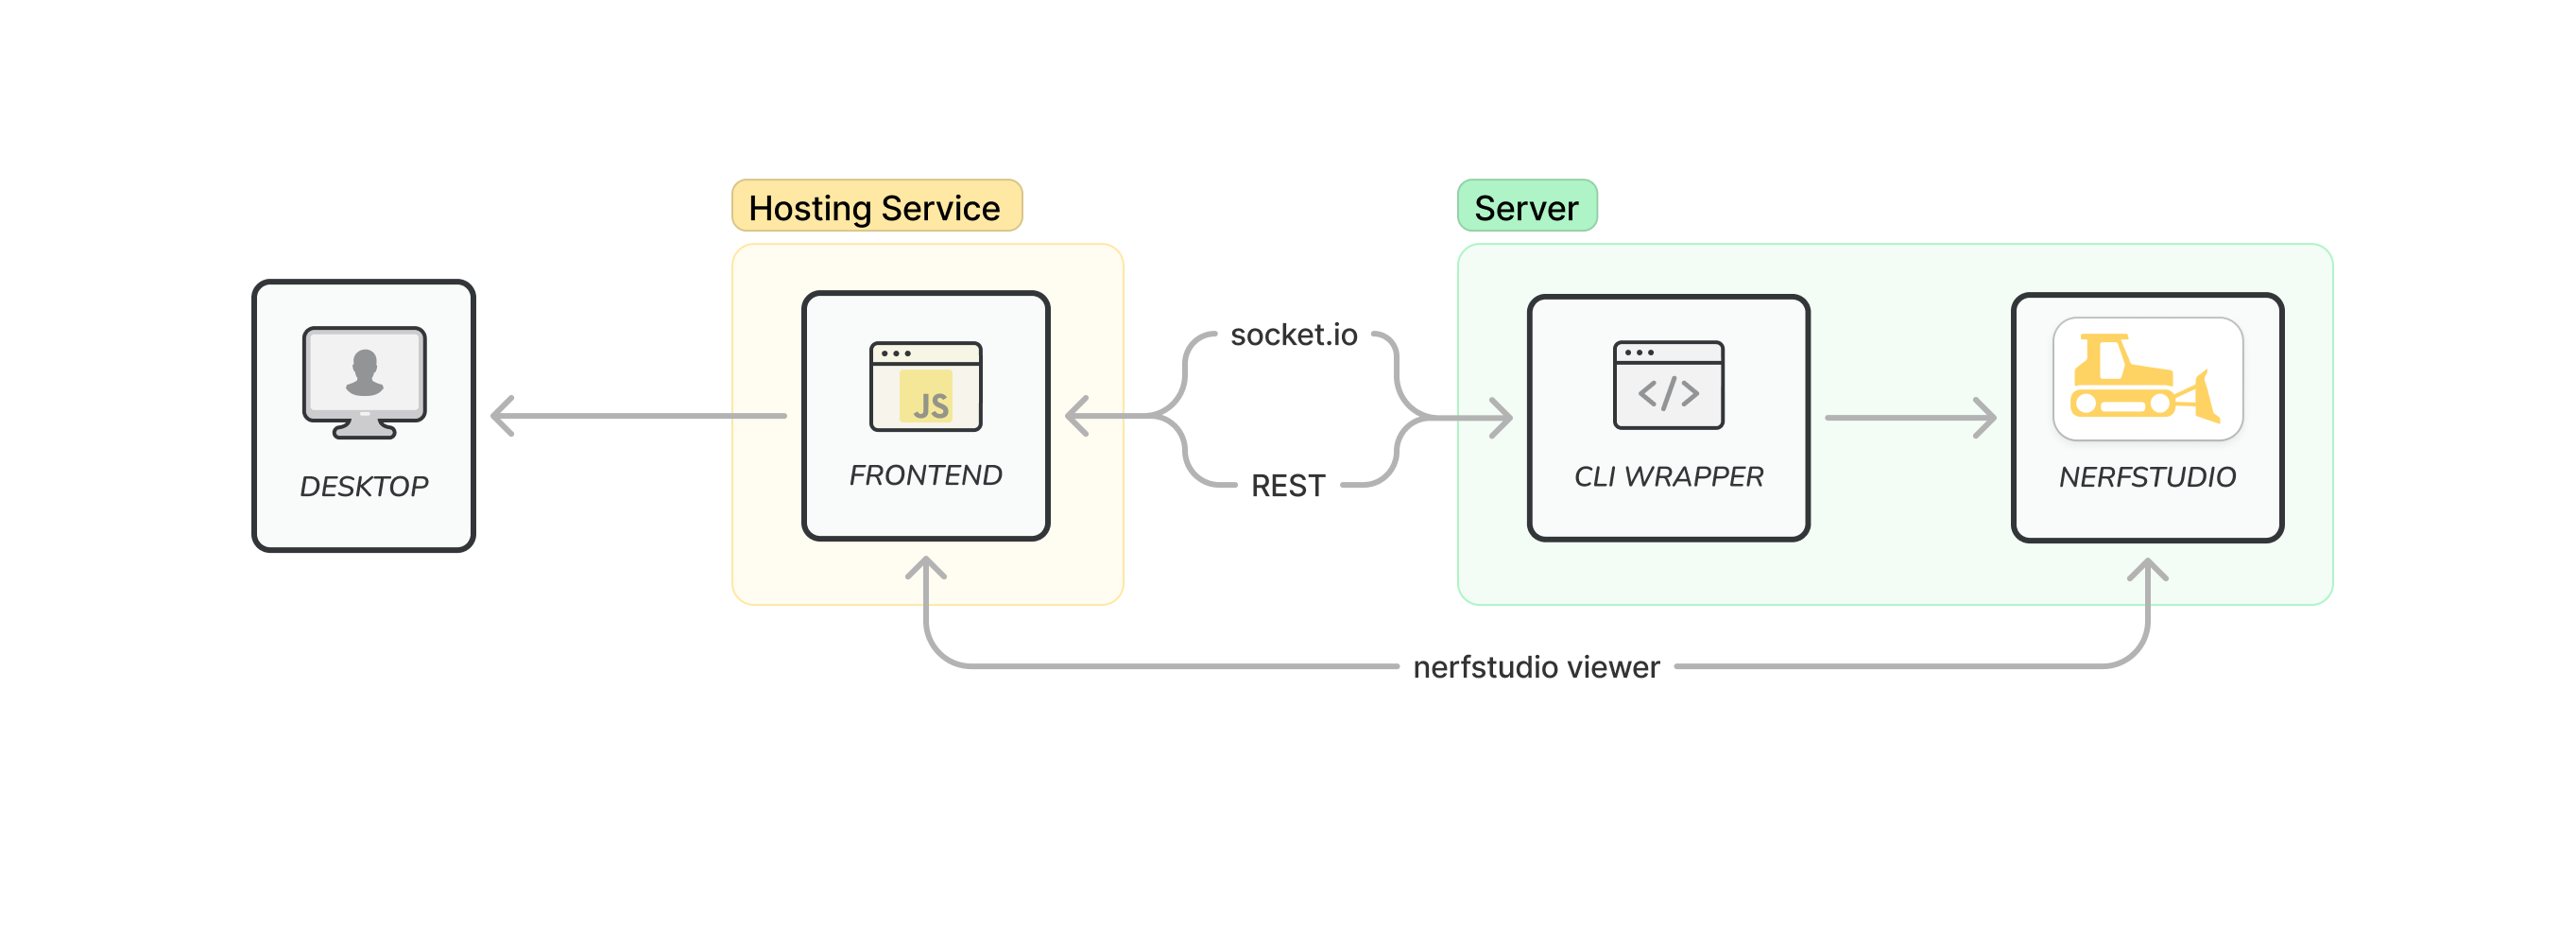
\includegraphics[width=\textwidth]{figures/architecture-1.png}
	\caption{System Architecture}
	\label{fig:system:example2}
\end{figure}

For the prototype, all the components were composed into a single docker container and deployed as a single unit.
This leveraged the pre-configured container provided by nerfstudio, and allowed for a quick and easy deployment of the prototype.

\section{Frontend Development} 
\label{sec:system:frontend}

% Setup, configuration, and component architecture
% UI/UX design principles

The frontend was built with React, as it is a popular and well supported framework for building web applications.
Vite was used as a build tool, as it provides a fast and efficient development experience.
To accelerate the styling process, Tailwind CSS was used, it is a utility-first CSS framework that provides a set of pre-defined classes that can be used to style components.
In additional the daisyUI component library provided a set of pre-styled components that could be used to quickly build the UI.

\subsubsection{Extensibility}

Extensibility was a key considerations during the development of the frontend, as the underlying nerfstudio CLI is in itself extendable.
All parameters for processing and training a NeRF model are configurable using JSON or strongly typed TypeScript objects.

\begin{lstlisting}[caption=Parameter Option configuration]
const stepsPerSave: NumberInput = {
	name: "stepsPerSave",
	label: "Steps Per Save",
	tooltip: "Number of steps between each save of the model.",
	inputType: "number",
	defaultValue: 1000,
};
\end{lstlisting}

Currently the supported input types are: number, select and boolean, but it is easy to add new types by extending the configuration object. 
It is also possible to define dependent parameters, that are only shown when a certain condition is met.
Images to illustrate the effect of a parameter can be added as well, to provide additional context to the user.

Filters and presets are also configurable using arrays of the names of the parameters that should be included in the filter or preset.
The full configuration can be found in the \texttt{frontend/src/config} folder in the codebase.

\subsubsection{Nerfstudio Viewer Integration}

The nerfstudio viewer is built using Viser, a library for building 3D visualizations using python.
This posed some limitations in integrating it into the frontend, as it is not easily possible to directly embed a python application into a web application.
To work around this, the viewer was hosted by nerfstudio as usual and embedded into the frontend using an iframe.

Some modifications could be made to the viewer to make it more suitable for embedding.
This included some simple styling changes to make the viewer fit better into the frontend.
The viewer contained several interactions where it was necessary for the user to copy console commands, to be used in the CLI.
These interactions were replaced with buttons that send a request to the server to execute the command instead.

These modifications were done at build-time of the container by applying a patch to the nerfstudio source code of the base image.


\section{Backend Development}
\label{sec:system:backend}

% Advantages of tRPC, configuration, and API design

The backend was built using tRPC, a framework for building type-safe APIs in TypeScript.
This type-safety was useful in building the API, as nerfstudio endpoints require a specific set of parameters of various types, that could be easily defined using TypeScript and reused in the frontend.

With tRPC, 

\section{Challenges and Solutions}
\label{sec:system:challenges}


\section{Lessons Learned}
\label{sec:system:lessons}

\section{Future Directions}
\label{sec:system:future}
         % INCLUDE: system
% !TEX root = ../main.tex
%
\chapter{User Study and Evaluation}
\label{sec:study}

To evaluate the usability and overall utility of the developed NeRF interface prototype, a comprehensive user study was conducted. 
The primary aim of this study was to collect feedback on the prototype's user experience, identify any usability challenges participants encountered, and understand their satisfaction levels with the interface. 
Employing a mixed-methods approach allowed for a blend of quantitative and qualitative data collection and analysis, offering a multifaceted view of the prototype's performance in real-world tasks.

Participants were given a set of tasks to complete within the prototype, followed by a User Experience Questionnaire (UEQ) and a follow-up interview to gather detailed feedback on their experiences.

\section{Participant Selection Criteria}
\label{sec:study:criteria}

Participants were selected in a similar fashion to the initial user research phase, with a focus on individuals working in the film industry and possessing varying levels of experience with NeRF technology, including none at all.

\begin{figure}[htb]
  \centering
  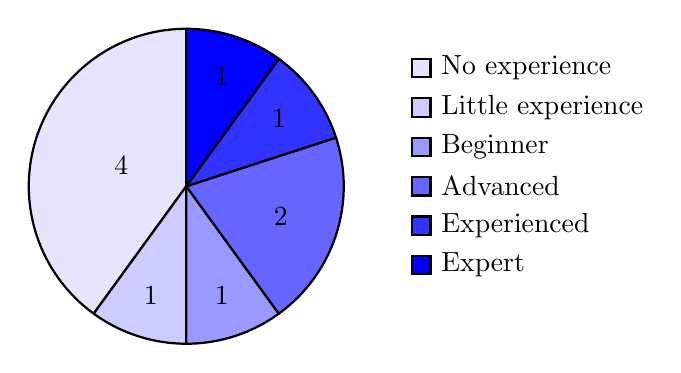
\begin{tikzpicture}
    \pie[sum=auto, text=legend, radius=2, rotate=90, color={blue!10, blue!20, blue!40, blue!60, blue!80, blue!100}]{4/No experience, 1/Little experience, 1/Beginner, 2/Advanced, 1/Experienced, 1/Expert }
  \end{tikzpicture}
  \caption{Participant Experience Levels}
  \label{fig:study:experience}  
\end{figure}

\section{Tasks Based Usability Test}
\label{sec:study:tasks}

The usability test was conducted in a controlled environment, with participants being asked to complete a two tasks with the prototype.
The tasks were designed to cover a range of functionalities and features of the prototype, and represent a typical workflow when creating NeRF models.

\begin{enumerate}
  \item Task: Create a new project.
  \item Task: Upload a prepared video file.
  \item Task: Pre-process the uploaded file to prepare it for training.
  \item Task: Switch to an existing project that already pre-processed data.
  \item Task: Start a NeRF training.
  \item Task: Create a camera path in the viewer.
  \item Task: Export a video.
\end{enumerate}

To keep an appropriate time frame, none of the tasks required completion of a training process, and pre-processed data and pre-trained models were provided to the participants.
On average, participants took 30 minutes to complete the tasks.

Participant were passively observed while working on their tasks, to identify any problems or operation errors they encountered and to determine their overall performance.
In addition the screen was recorded to capture the participants interactions with the prototype, and to allow for a more detailed analysis of their behavior later on.

\section{User Experience Questionnaire}
\label{sec:study:ueq}

After completing their tasks, users were asked to fill out the User Experience Questionnaire (UEQ) \cite{laugwitz_construction_2008}, a standardized questionnaire for the assessment of user experience.
The placement of the UEQ after the tasks was chosen to capture the immediate impressions of the participants, while the experience was still fresh in their minds and without being influenced by the follow-up interview.
It measure user experience in six dimensions:

\begin{itemize}
  \item \textbf{Attractiveness} - the overall impression of the product
  \item \textbf{Perspicuity} - the clarity and understandability of the product
  \item \textbf{Efficiency} - the perceived effort required to use the product
  \item \textbf{Dependability} - the perceived reliability and trustworthiness of the product
  \item \textbf{Novelty} - the perceived originality and innovation of the product
  \item \textbf{Stimulation} - the perceived level of excitement and engagement with the product
\end{itemize}

This covers both classical usability goals (Efficiency, Perspicuity, Dependability) and user experience qualities (Novelty, Stimulation).
Attractiveness is purely a valence dimension, and is not directly related to usability or user experience.

In total the questionnaire consists of 26 items, each represented by two terms of opposite meaning. 
The order of the terms is randomized for each item, to avoid bias.
Participants are asked to rate each item on a 7-point scale, from -3 to +3, with 0 representing a neutral response.
An example of the scale can be seen below:

\begin{center}
  boring \quad o o o o o o o \quad exciting
\end{center}

The format of the questionnaire gives participants a clear and simple way to  quickly express their feelings and thoughts about the prototype, without much effort.

In this study the questionnaire was filled out by participants in digital form, using a web-based survey tool. \todo{source}
The survey included additional questions to gather demographic information and to capture prior experience with NeRF and other 3D modeling tools.
This allowed for a more efficient data collection and analysis, across in-person and remote participants.

\section{Follow-up Interview}
\label{sec:study:interview}

After completing the usability test, participants were engaged in a short follow-up interview, to gather more detailed feedback on their experience with the prototype. 
Similar to the initial user interviews, these interviews were semi-structured, following a pre-defined set of question, with room for participants to share their own thoughts and suggestions.
The questions can be categorized into general usability, tasks specific feedback and suggestions for improvement.
The interview template can be found in the appendix \ref{sec:appendix:questionnaire}.


\section{Data Analysis}
\label{sec:study:analysis}

Both the recordings of the usability test and the follow-up interviews were analyzed to identify common themes and patterns in the feedback of participants.
The video recordings were coded to highlight any usability issues or challenges that participants encountered during the tasks.
The audio recordings of the interviews were transcribed and coded.
The data was then categorized and analyzed to identify common themes and patterns across the participants.

Analysis of the UEQ data was done using the standard procedure for the questionnaire.
The UEQ provides a data analysis tool in form of spreadsheet, that calculates all necessary values and visualizes the results.

In summary, this user study and evaluation was pivotal in validating the effectiveness of the NeRF interface prototype, uncovering valuable insights into its usability, and identifying opportunities for further refinement. 
The mixed-methods approach ensured a balanced assessment, capturing both the tangible aspects of interface interaction and the subjective experiences of the users, providing a solid foundation for the next stages of development.

% !TEX root = ../main.tex
%
\chapter{Results}
\label{sec:result}


\section{Analysis of User Experience Questionaire}
\label{sec:result:ux}


\section{Findings from Qualitative User Testing}
\label{sec:result:testing}


\section{Integration and Findings}
\label{sec:result:findings}

         % INCLUDE: system
% !TEX root = ../main.tex
%
\chapter{Discussion}
\label{sec:discussion}

% TODO: Write discussion

% Interpretation of results in the context of existing NeRF creation methods
% Implications for the film and VFX industry
% Discussion on the integration of user feedback into the prototype
% Limitations of the study and the prototype

\section{Interpretation of Results}
\label{sec:discussion:results}

\section{Implications for the Film and VFX Industry}
\label{sec:discussion:implications}

\section{Integration of User Feedback}
\label{sec:discussion:user-feedback}

Based on the issues identified during user testing, several adjustments were made to enhance the usability and intuitiveness of the application. These changes are outlined below:

\paragraph{Improved Navigation}
To address the confusion in navigation to the dashboard (\ref{sec:results:issues:navigation}), a dedicated button was added to the navigation bar. 
This feature has should improved the clarity of  navigation to users significantly. \fref{fig:fix-1}

\begin{figure}[htb]
  \centering
	
\includegraphics[width=0.5\textwidth]{figures/fix-1.png}
	\caption{Dedicated Button for Dashboard Navigation}
  \label{fig:fix-1}
\end{figure}

\paragraph{Clarified Wording}
The wording on the button to start the training process was changed from \emph{"Start Processing"} to \emph{"Start Training"}, which aligns better with user expectations and reduces confusion. \fref{fig:fix-2}

\begin{figure}[htb]
	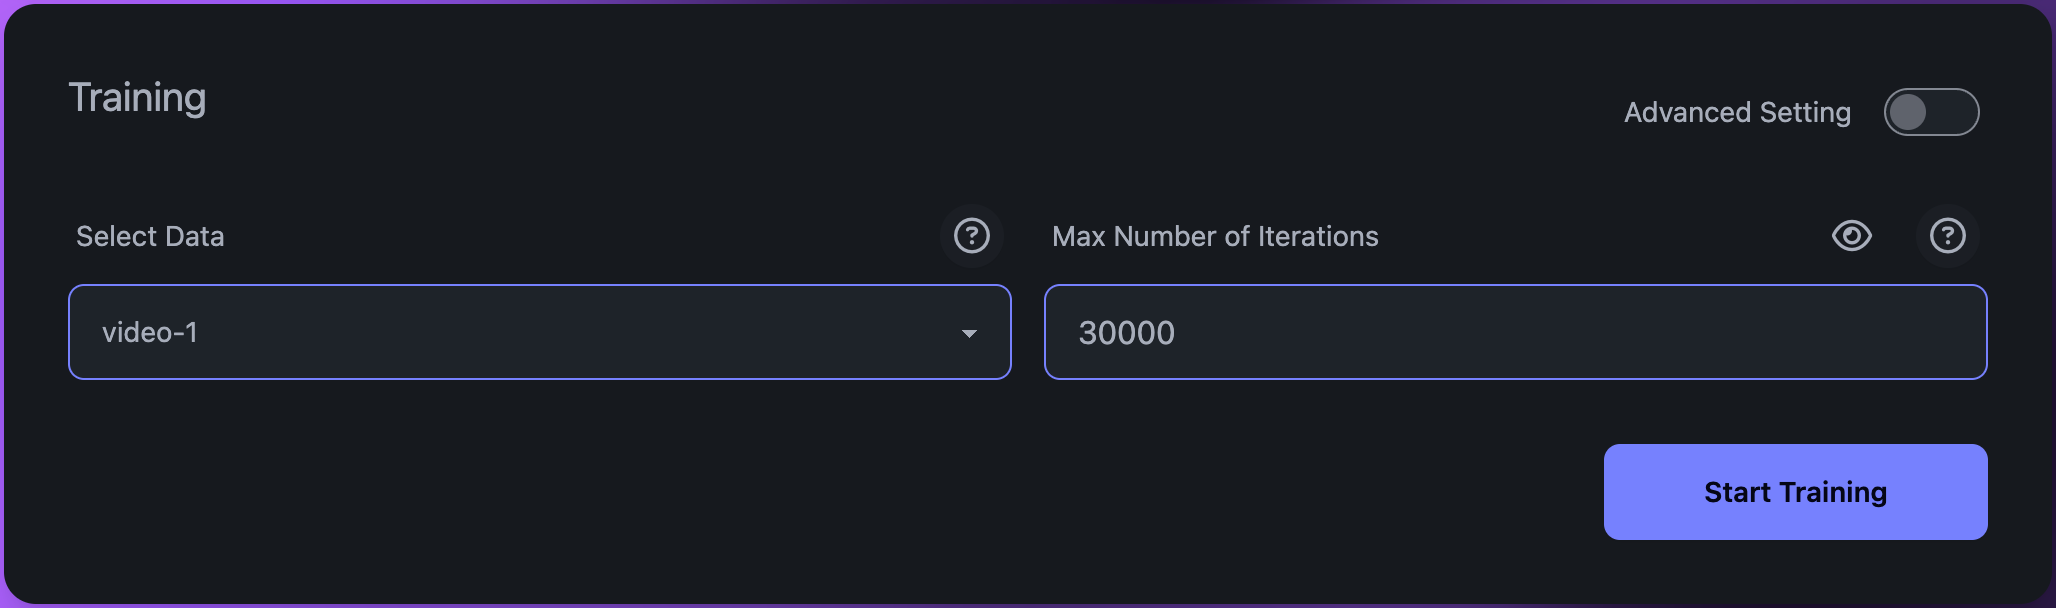
\includegraphics[width=\textwidth]{figures/fix-2.png}
	\caption{Consistent Wording for Training Button}
  \label{fig:fix-2}
\end{figure}

\paragraph{Enhanced Project Creation}
The project creation process was moved into a modal dialog, which not only eliminates a point of confusion but also clarified the need to name projects before creation. \fref{fig:fix-3}

\begin{figure}[htb]
	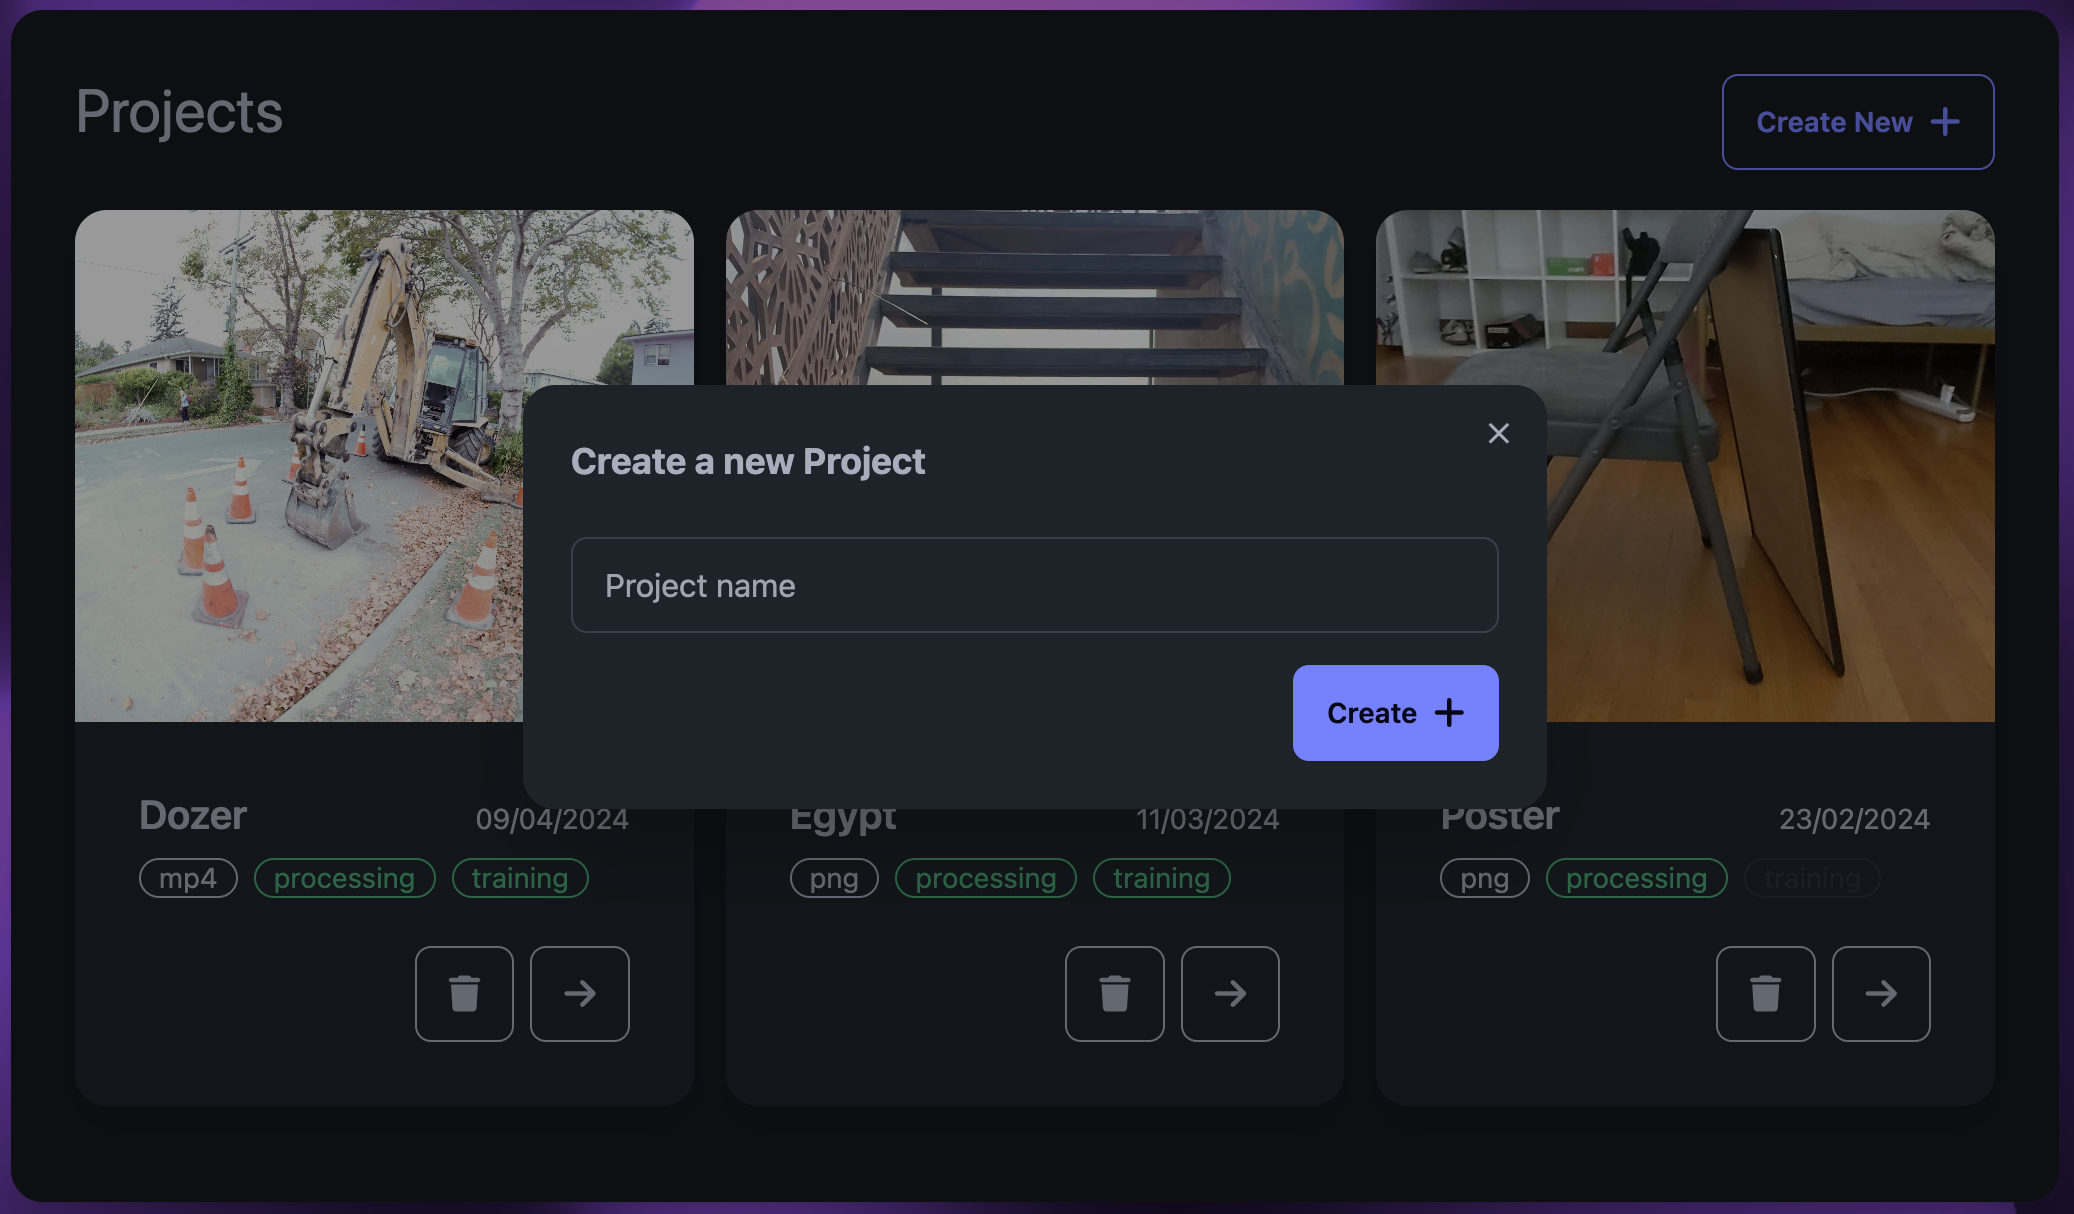
\includegraphics[width=\textwidth]{figures/fix-3.png}
	\caption{Modal Dialog for Project Creation}
  \label{fig:fix-3}
\end{figure}

\paragraph{File Upload Improvements}
The file upload process was improved by adding some guardrails, to ensure user would not accidentally skip a step. 
The upload button starts out disabled, so that the only interactive element is the file-input field.
Once a file is selected, the button becomes active, indicating to the user that they can proceed to upload their selected file.
Only one the file is uploaded, the UI elements related to pre-processing appear, guiding the user through the next steps. 
This solution is likely to prevent many of the issues users encountered when uploading files during testing. \fref{fig:fix-4}


\begin{figure}[htb]
  \begin{subfigure}{\textwidth}
    \centering
    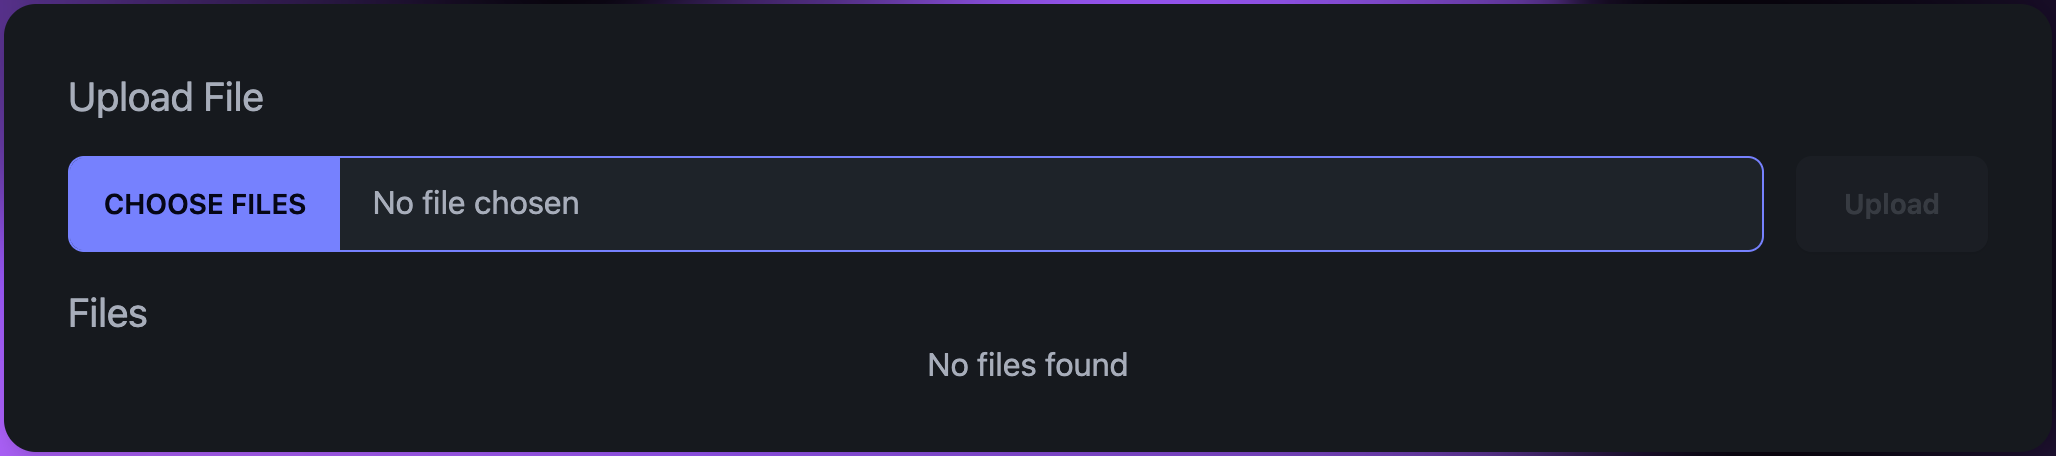
\includegraphics[width=.8\linewidth]{figures/fix-4.1.png}
    \caption{Initial State}
  \end{subfigure}
  \begin{subfigure}{\textwidth}
    \centering
    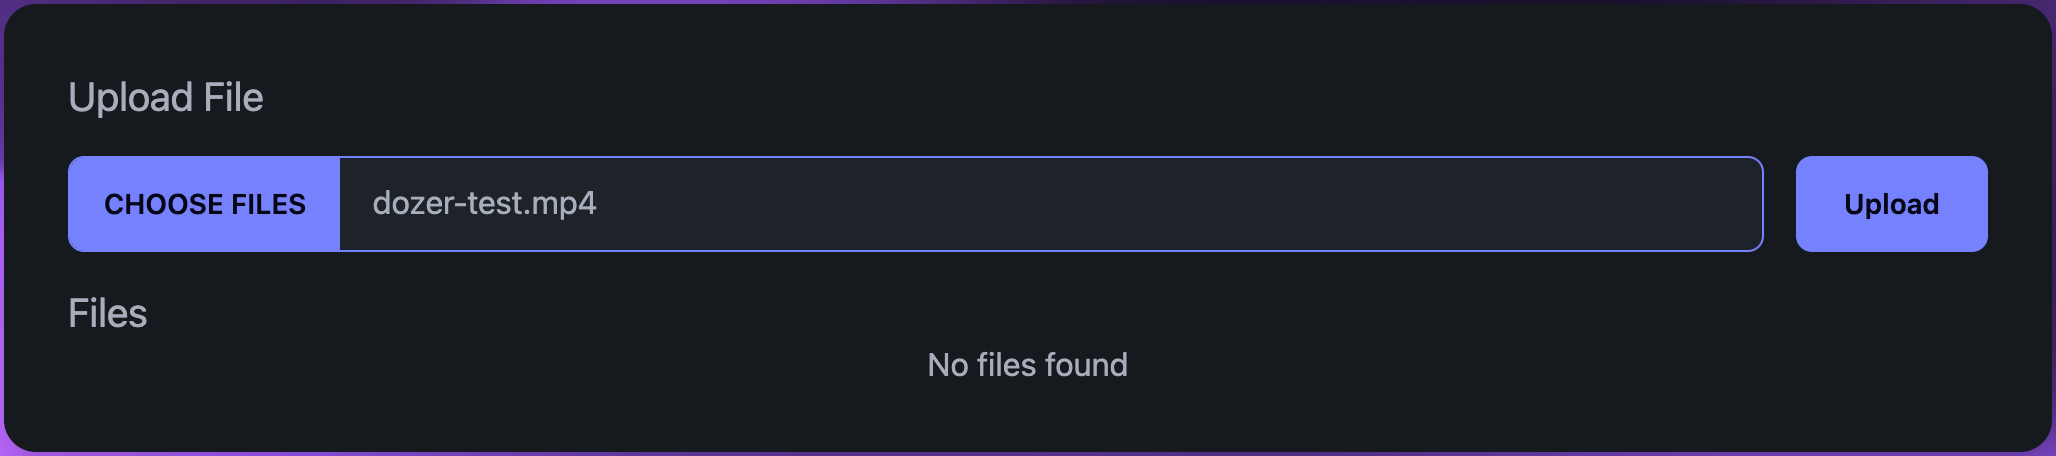
\includegraphics[width=.8\linewidth]{figures/fix-4.2.png}
    \caption{File Selected}
  \end{subfigure}
  \begin{subfigure}{\textwidth}
    \centering
    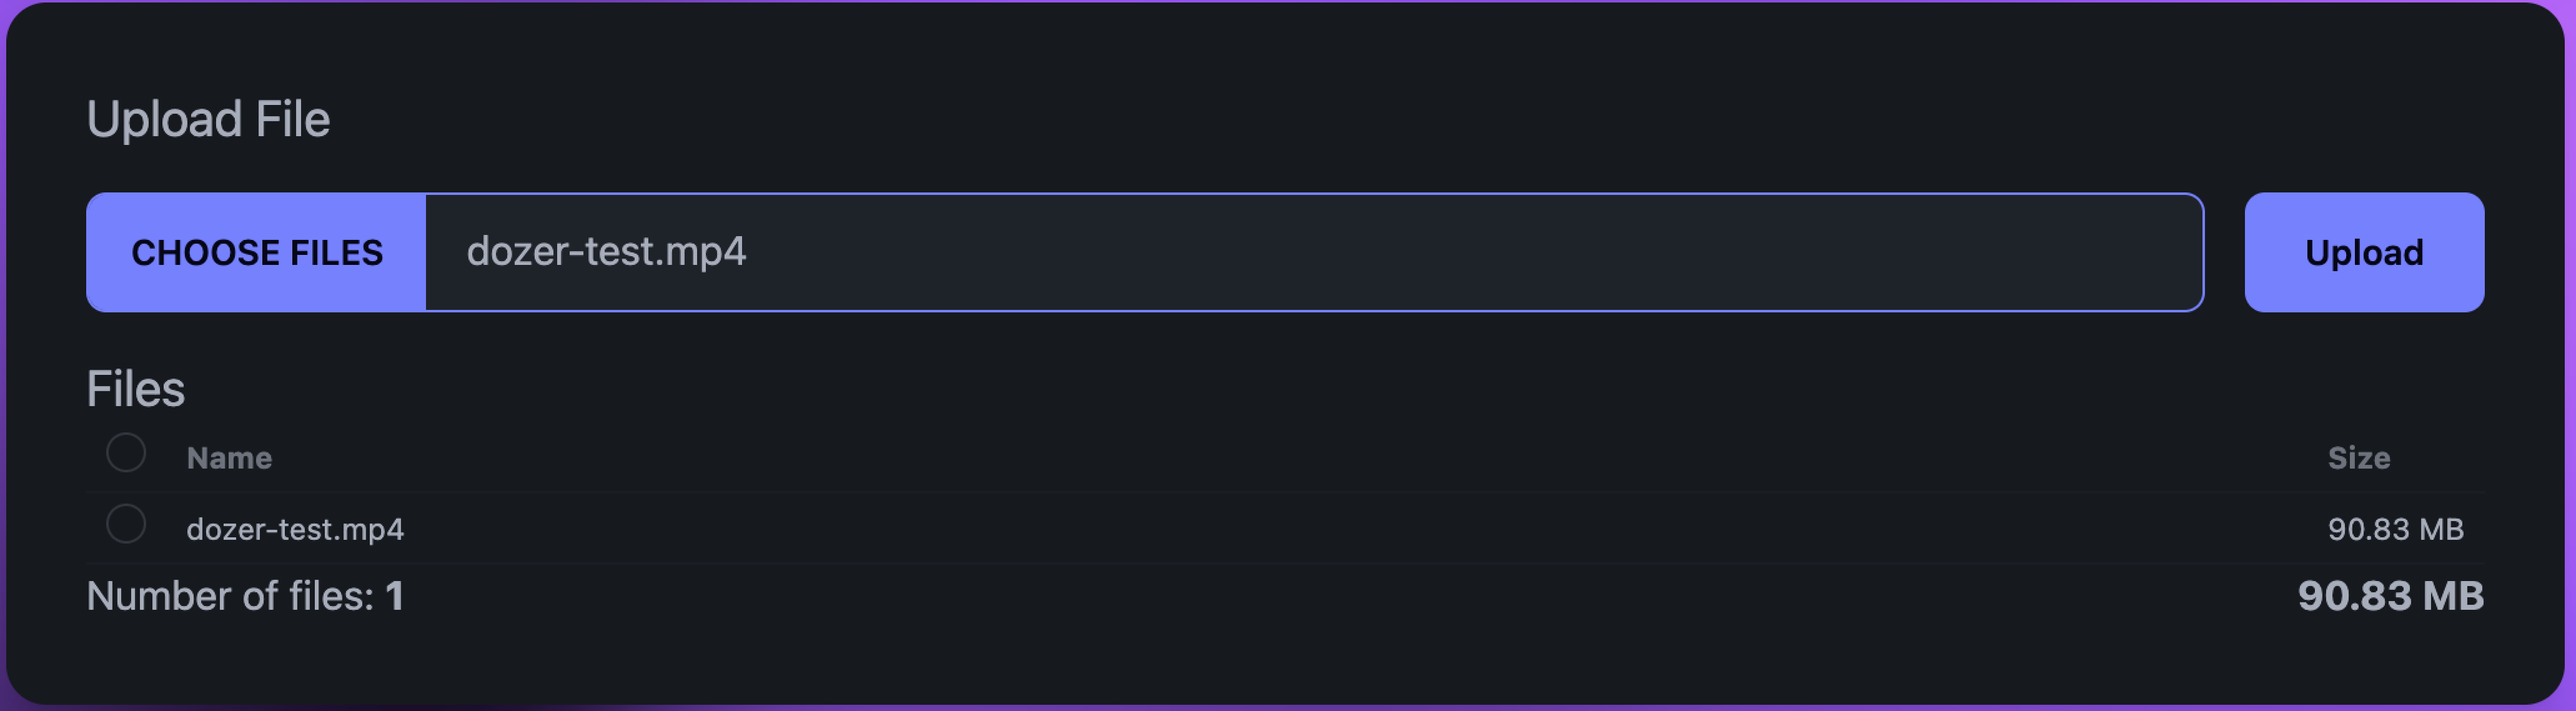
\includegraphics[width=.8\linewidth]{figures/fix-4.3.png}
    \caption{File Uploaded}
  \end{subfigure}
	\caption{Improved File Upload Process}
  \label{fig:fix-4}
\end{figure}

\section{Limitations}
\label{sec:discussion:limitations}

% !TEX root = ../main.tex
%
\chapter{Conclusion}
\label{sec:conclusion}
% TODO: Write conclusion

\section{Key Findings}
\label{sec:conclusion:findings}

\section{Contributions to the Field}
\label{sec:conclusion:contributions}

\section{Future Work}
\label{sec:conclusion:future}

     % INCLUDE: conclusion

% --------------------------
% Back matter
% --------------------------
\appendix\cleardoublepage
% !TEX root = ../main.tex
%
\chapter{Example Appendix}
\label{sec:appendix}

\Blindtext[1][1]

\section{Appendix Section 1}
\label{sec:appendix:sec1}

\Blindtext[1][1]

\begin{table}[h]
	\begin{tabularx}{\textwidth}{X | X | X}
		%\hline
		Alpha		& Beta			& Gamma			\\ \hline
		0			& 1				& 2				\\ \hline
		3			& 4				& 5				\\ %\hline
	\end{tabularx}
	\label{tab:table1}
	\caption{This is a caption text.}
\end{table}

\section{Appendix Section 2}
\label{sec:appendix:sec2}

\Blindtext[1][1]

\begin{table}[h]
	\begin{tabularx}{\textwidth}{X | X | X}
		%\hline
		Alpha		& Beta			& Gamma			\\ \hline
		0			& 1				& 2				\\ \hline
		3			& 4				& 5				\\ %\hline
	\end{tabularx}
	\label{tab:table2}
	\caption{This is a caption text.}
\end{table}

\Blindtext[1][2]
       % INCLUDE: appendix
%
{%
\setstretch{1.1}
\renewcommand{\bibfont}{\normalfont\small}
\setlength{\biblabelsep}{0pt}
\setlength{\bibitemsep}{0.5\baselineskip plus 0.5\baselineskip}
\printbibliography[nottype=online]
\newrefcontext[labelprefix={@}]
\printbibliography[heading=subbibliography,title={Webpages},type=online]
}

\listoffigures

\listoftables

% **************************************************
% End of Document CONTENT
% **************************************************
\end{document}
